\documentclass{tietreport}

\usepackage{graphicx}
\usepackage{amsmath,amssymb}
\usepackage{booktabs}
\usepackage{array}
\usepackage{tabularx}
\usepackage{xltabular}
\usepackage{float}
\usepackage{tikz}
\usetikzlibrary{arrows.meta,positioning,shapes.geometric,shapes.multipart,calc,fit,backgrounds,patterns}
\usepackage{pgfplots}
\pgfplotsset{compat=1.17}

\usepackage[date=year,style=alphabetic,backend=biber,sorting=nty,maxnames=5,minnames=3,
  maxalphanames=4,minalphanames=3,backref=true,doi=false,isbn=false,url=false,eprint=false]{biblatex}
\addbibresource{references.bib}
\IfFileExists{tfrupee.sty}{\usepackage{tfrupee}}{\newcommand{\rupee}{Rs.~}}

\makeatletter
\@ifpackageloaded{hyperref}{\hypersetup{hidelinks}}{}%
\AtBeginDocument{\@ifpackageloaded{hyperref}{\hypersetup{hidelinks}}{}}%
\makeatother

\newcolumntype{L}[1]{>{\raggedright\arraybackslash}p{#1}}
\newcolumntype{Y}{>{\raggedright\arraybackslash}X}

\tikzset{
  umlclass/.style={draw, rectangle split, rectangle split parts=#1, rectangle split part align={center,left,left},
    font=\scriptsize\ttfamily, text width=41mm, inner sep=3pt, align=left,
    rectangle split part fill={black!8,white,white}},
  umlclass/.default=3,
  inherit/.style={-{Triangle[open,length=3mm,width=3mm]}, thick},
  assoc/.style={-{Latex[length=2mm]}, thick},
  compose/.style={{Diamond[fill=black,length=3mm,width=2mm]}-{Latex[length=2mm]}, thick},
  aggreg/.style={{Diamond[open,length=3mm,width=2mm]}-{Latex[length=2mm]}, thick},
  depend/.style={-{Latex[open,length=2mm]}, thick, dashed},
  actor/.style={font=\scriptsize, align=center, inner sep=1pt},
  usecase/.style={draw, ellipse, font=\scriptsize, align=center, inner sep=2pt, minimum width=28mm, minimum height=9mm, fill=white},
  swim/.style={draw, dashed, gray!70, inner sep=6pt},
  swimlabel/.style={font=\footnotesize\bfseries, anchor=north west, inner sep=3pt},
}

%% ================= TITLE PAGE FIELDS =================
\TitlePageHeader{UCS503 - Software Engineering}
\ProjectTitle{Adaptive AI Interviewer}
\ProjectSubTitle{An Item-Response-Theory Based Adaptive Assessment Engine for Technical
  Interviews: Requirements, Feasibility, Foundations, Hybrid Retrieval and the Adaptive Core (Phases 1--3)}
\author{\texttt{1024030854} Bhavik Gupta}
\TitlePageSubText{Group: \texttt{3C62} BE Third Year, CSE}
\AdvisorName{Ms. Reaya Grewal}
\TitlePageFooterText{{\large Mid-Semester Evaluation \\[0.2cm]
    \bfseries Computer Science and Engineering Department} \\[0.15cm]
  Thapar Institute of Engineering and Technology, Patiala}

\begin{document}
\maketitle
{\small\setcounter{tocdepth}{1}\tableofcontents}

% =====================================================================
\chapter{Introduction}
\label{ch:intro}

\section{Background and Context}

Automated technical interviewing is a crowded category, and most systems in it share one
design: a large language model (LLM) is prompted to ask a question, read the answer, and
produce a score. Such a system has no measurement model. It cannot say how confident it is
about a candidate, cannot explain why it asked a particular question, and cannot be
reproduced, because every decision lives inside a prompt.

This project takes the opposite position. It is a \emph{computerised adaptive testing} (CAT)
engine \cite{vanderlinden2000cat,lord1980irt} for technical interviews, in which a candidate's
ability on each skill is a latent variable $\theta$ estimated from evidence, each question
carries a calibrated difficulty $b$ on the same scale, and the next question is chosen to
maximise the information gained about $\theta$ subject to coverage constraints derived from
the job description. The LLM is confined to three jobs -- \emph{understand} (parse a resume or
job description), \emph{judge} (classify an answer against a concept checklist) and
\emph{speak} (phrase questions and follow-ups). It never decides control flow and it never
emits a score; all arithmetic happens in code. That single decision is what makes the system
testable, reproducible, inexpensive and structurally resistant to prompt injection, and what
allows the central question -- \emph{does adaptive selection measure a candidate better than a
non-adaptive one?} -- to be asked as an experiment rather than asserted.

The work is a 45-day, nine-phase solo build. This report covers \textbf{Phases 1--3 (Days
1--15)}: the foundations and the LLM chokepoint, the question bank and hybrid retrieval, and
the adaptive engine (ability estimation, item selection, simulation, convergence analysis and
the assessment blueprint). No grading pipeline, session API, front end or deployment exists
yet; those are Phases 4--9.

\subsection{Problem Statement}

Given a job description with weighted topic requirements, a time budget, and a bank of
questions with calibrated difficulty and expected-concept checklists, the system must:
(1)~maintain a per-subtopic estimate of ability $\theta$ with an honest uncertainty RD, updated
from graded answers; (2)~choose at every turn the most informative question while respecting
hard constraints (no repeats, topic quotas, a difficulty window, the remaining clock);
(3)~stop when the estimate is precise enough, the budget is spent, or answers stop carrying
information; (4)~retrieve questions by meaning and keyword with measured ranking quality; and
(5)~route every LLM call through a single validated, cost-accounted, fail-over-capable
chokepoint. The specific difficulty is validation: an adaptive engine will always produce
\emph{a} question and \emph{a} score, so the ability model and selection policy are built as
pure functions and measured in a simulation with known ground truth before any real candidate
exists.

\section{Motivation and Need Analysis}

Placement season compresses months of preparation into a few weeks, and the practice
available to a student comes in two kinds. Fixed question sets are cheap and repeatable but
ask the same thirty questions of a strong and a weak candidate, spending most of their length
on items too easy or too hard to be informative. Human mock interviews adapt well but are
scarce, inconsistent and unavailable at scale. An adaptive assessment sits between the two:
every question is chosen because it is the one most likely to change what the system believes,
and the interview stops when there is nothing left to learn. The theory has existed for
decades and underpins large-scale examinations, but it has not been applied to open-ended
technical interviews because, until recently, nothing could read a free-text answer and say
which expected concepts it contains. Language models can now do that reading; what they cannot
do reliably is the arithmetic. The project's motivation is the combination: the model for
reading, judging and phrasing; deterministic, testable code for every number.

\section{Project Objectives}

The objectives are the phase exit gates from the project plan, each a pass/fail criterion.
\begin{enumerate}
  \item \textbf{Phase 1 -- Foundations:} a clean clone boots to a working API with
    \texttt{docker compose up}; register $\to$ login $\to$ authenticated \texttt{/me} works; one
    LLM call succeeds through the single chokepoint and appears in tracing with its cost; a dead
    primary provider fails over automatically, proven by a test; CI is green.
  \item \textbf{Phase 2 -- Question bank and retrieval:} 150 reviewed bank items passing CI
    validation; a search endpoint returning ranked results in under 300\,ms; a four-row ablation
    table (vector / lexical / hybrid / hybrid+rerank) on a labelled query set.
  \item \textbf{Phase 3 -- Adaptive engine:} a tested ability model including property tests; a
    convergence chart generated by a committed script; and \emph{adaptive selection reaching a
    given precision in materially fewer items than random selection} in simulation.
\end{enumerate}
Objective~1 is met. Objective~2 is partially met (60 of 150 items, none human-reviewed; the
HTTP endpoint is not built). Objective~3 is met on two of three gates; the third is
\textbf{not met}, and Chapter~\ref{ch:results} presents the evidence in full.

\section{Scope, Stakeholders and Constraints}

\paragraph{In scope for this evaluation.} A containerised, authenticated FastAPI service; a
single validated chokepoint for every LLM call with retry, failover, a circuit breaker and an
offline replay provider; a validated question bank with a taxonomy and expected-concept
checklists, embedded and lexically indexed in PostgreSQL with hybrid retrieval and a labelled
evaluation; the adaptive engine (ability model, selector, stopping rule, blueprint) as pure
functions; and a zero-token simulation comparing adaptive, random and fixed policies.

\paragraph{Planned (Phases 4--9).} The grader with a 120-answer labelled validation set and
prompt-injection suite (4); session orchestration over an event log, resume/JD parsing with PII
redaction, the report pipeline (5); a React front end and public deployment, Version~1 (6); a
sandboxed coding round (7); subscriptions and metering, Version~2 (8); an agentic round,
difficulty calibration and documentation, Version~3 (9).

\paragraph{Non-goals.} The system is a \emph{practice} tool. It does not make or recommend
hiring decisions, never auto-rejects anyone, and its report says what to study next rather than
ranking people. Version~1 is English-only and text-only.

\paragraph{Stakeholders.} The \emph{candidate} (a student preparing for placements) needs a
short adaptive interview and an honest, evidence-backed, non-judgemental per-skill report with
privacy for their resume and answers. The \emph{assessment author} (a mentor, TA or the
candidate) turns a job description and time budget into a blueprint. The \emph{bank author}
writes and reviews items that must pass validation. The \emph{developer} needs a system that is
testable offline, reproducible and cheap. The \emph{faculty guide} needs evidence that gates are
recorded truthfully. The \emph{LLM provider} is an external system reached only through the
chokepoint.

\paragraph{Assumptions.} Ability per subtopic is one-dimensional and the two-parameter
logistic model is a workable approximation \cite{vanderlinden2000cat}; hand-authored $b$ and $a$
are treated as correct until calibrated (Phase~9); a schema-constrained LLM can classify concept
coverage at quadratic-weighted kappa $\geq 0.65$ against human labels (the Phase~4 gate, and the
single most important unverified assumption); any free-tier provider can be down at any time.

\paragraph{Constraints.} One developer, 45 working days at 12--15 hours a week with a hard
mid-semester gate at Day~15; a near-zero cash budget with a default test suite that needs no
network, database, model download or API key; a laptop CPU and no GPU; PII stripped from
resumes before any text reaches a model; nothing pushed publicly or deployed before Day~30.

% =====================================================================
\chapter{Literature Review and Existing Systems}
\label{ch:literature}

\section{Existing Systems}

Interview-preparation tools fall into four categories. \emph{Fixed online assessments} (the HackerRank / LeetCode style) are cheap and repeatable but give every candidate the same sequence and cannot grade open-ended answers. \emph{Peer and expert mock interviews} (the Pramp / interviewing.io style) adapt well but are scarce, inconsistent and unrepeatable. \emph{LLM-prompted interviewer bots} read free text but let the model both choose questions and emit the score inside a prompt, so decisions are unexplainable and open to injection. \emph{Computerised adaptive tests} have a rigorous psychometric model \cite{vanderlinden2000cat} but only for closed-form items. The gap is the intersection: the rigour of the fourth applied to the open-ended content of the first two, with the reading ability of the third confined to the one place it is needed.

\section{Item Response Theory and Adaptive Testing}

Item response theory models the probability that a person of ability $\theta$ answers an item
of difficulty $b$ correctly as a monotone function of $\theta-b$; Lord \cite{lord1980irt} is the
standard treatment of the two-parameter logistic model used here. Weiss and Kingsbury
\cite{weiss1984cat} showed adaptive tests reach a given precision with substantially fewer items
than fixed tests -- the claim this project set out to test in its own domain. Van der Linden and Glas \cite{vanderlinden2000cat} collect selection, content balancing, exposure control and stopping rules, of which the project's hard-constraint filters and $\varepsilon$-greedy draw are simple instances. Instead of maximum-likelihood estimation, the engine uses an Elo-style incremental update
\cite{elo1978rating} -- one gradient step on the logistic log-loss -- paired with Glickman's
rating deviation \cite{glickman1999glicko} for an explicit, shrinking uncertainty; Pel\'anek
\cite{pelanek2016elo} documents this family succeeding in adaptive educational systems.

\section{Retrieval, LLM Judges and Their Failure Modes}

Dense retrieval uses the BGE bi-encoders \cite{xiao2023cpack} over HNSW indexes \cite{malkov2020hnsw} in \texttt{pgvector}; lexical search is PostgreSQL full-text search; reciprocal rank fusion \cite{cormack2009rrf} merges the two using ranks alone; cross-encoder reranking \cite{nogueira2019bert} is the standard second stage; quality is measured with recall, MRR and nDCG \cite{jarvelin2002ndcg}.

Zheng et al.\  \cite{zheng2023judge} measured LLM judges at near human--human agreement while documenting position, verbosity and self-enhancement biases, and Greshake et al.\  \cite{greshake2023injection} showed LLM-integrated applications can be hijacked by instructions hidden in the data they read. Both shape the design: the model only classifies concept coverage with evidence spans, never emits a number, receives schema-constrained redacted inputs, and its evidence is verified as a substring of the original text in code.

% =====================================================================
\chapter{Requirement Analysis}
\label{ch:requirements}

Requirements were elicited from the technical blueprint written before Day~1, the feasibility study (Chapter~\ref{ch:feasibility}), conversations with peers preparing for placements, and the work itself. Status at Day~15 is \emph{Done}, \emph{Partial} or \emph{Planned}, filled from the evidence in Chapter~\ref{ch:results}.

\section{Functional Requirements}

{\footnotesize
\begin{xltabular}{\linewidth}{L{0.08\linewidth} Y L{0.06\linewidth} L{0.18\linewidth}}
\caption{Functional requirements delivered in Phases 1--3 (the grader, session API, resume parsing and report belong to Phases 4--6).}\label{tab:fr}\\
\toprule \textbf{ID} & \textbf{Requirement} & \textbf{Ph.} & \textbf{Status} \\ \midrule
\endfirsthead
\toprule \textbf{ID} & \textbf{Requirement} & \textbf{Ph.} & \textbf{Status} \\ \midrule
\endhead
\bottomrule
\endlastfoot
FR-01 & Register, log in, refresh and log out; the identity is available to every protected endpoint. & 1 & Done \\
FR-02 & Every LLM call passes through one function that validates the response against a schema, records tokens, latency and cost, and fails over between providers. & 1 & Done (live) \\
FR-03 & The system runs fully offline by replaying recorded provider answers, always distinguishable from live ones. & 1 & Done \\
FR-04 & Bank items carry taxonomy keys, calibrated $b$ and $a$, weighted expected concepts, misconceptions, a reference answer and review provenance; invalid items are rejected with every error listed. & 2 & Done (60/150) \\
FR-05 & Items are ingested idempotently with a dense embedding and a lexical index; unchanged items are not re-embedded. & 2 & Done \\
FR-06 & Questions are retrieved by meaning and keyword, fused, optionally reranked, and ranking quality is measured on a labelled set. & 2 & Done; no HTTP endpoint \\
FR-07 & Per subtopic, $\theta$ and RD are updated from a graded score and confidence and aggregated to topic and domain on read. & 3 & Done (97 tests) \\
FR-08 & The next question is selected from items satisfying all hard constraints, ranked by a documented objective with bounded exploration; every choice is explainable and a seeded session reproducible. & 3 & Done \\
FR-09 & The assessment stops on precision, item budget, time budget or no new information, reporting every reason that fired. & 3 & Done \\
FR-10 & A role, level, mode, duration and weighted topics become a validated, serialisable blueprint. & 3 & Done (226 tests) \\
FR-11 & The adaptive policy is compared against random and fixed policies on a synthetic population with known ground truth, without any model call. & 3 & Done \\
\end{xltabular}
}

\section{Non-Functional Requirements}

{\footnotesize
\begin{xltabular}{\linewidth}{L{0.08\linewidth} L{0.15\linewidth} Y L{0.17\linewidth}}
\caption{Non-functional requirements with status at Day 15.}\label{tab:nfr}\\
\toprule \textbf{ID} & \textbf{Category} & \textbf{Requirement} & \textbf{Status} \\ \midrule
\endfirsthead
\toprule \textbf{ID} & \textbf{Category} & \textbf{Requirement} & \textbf{Status} \\ \midrule
\endhead
\bottomrule
\endlastfoot
NFR-01 & Correctness & Every number shown to a user is computed in code, never by a language model. & Done by construction \\
NFR-02 & Reproducibility & Every experiment and figure regenerates byte-for-byte from a committed script and seed. & Done (tested) \\
NFR-03 & Testability & The default suite runs with no network, database, model or key; numerical modules are pure functions tested against hand-worked values. & Done (1,536 pass in $\sim$18\,s) \\
NFR-04 & Performance & Hybrid search under 300\,ms per query. & Done (58\,ms) \\
NFR-05 & Reliability & Dead providers fail over; repeat failures are circuit-broken; the API never serves an un-migrated schema. & Done (unit and live) \\
NFR-06 & Security & argon2id; short-lived access tokens; single-use rotating refresh tokens with reuse detection; lock-out; no secret in any log; gitleaks in CI. & Done (verified on real logs) \\
NFR-07 & Privacy & PII stripped before any text reaches a model; encryption at rest; retention limit; working delete. & Planned (Phase~5) \\
NFR-11 & Maintainability & \texttt{ruff}, \texttt{mypy --strict} and the suite clean on every commit; docstrings and ADRs as design records. & Done \\
N\end{xltabular}
}

\section{Interfaces, Data and Risks}

No graphical interface exists yet; the system is operated through the HTTP API, command-line scripts (validate, ingest, evaluate, simulate) and the test suite. PostgreSQL with \texttt{pgvector}, Redis, the OpenAI-compatible chat endpoint and the ONNX runtime each sit behind an interface with a stub or fallback; no GPU is assumed. Persistent data (accounts, taxonomy, questions, skill states, sessions, events, turns) is described in Section~\ref{sec:data-design}; turns and resumes are the most sensitive and are deletable.

Table~\ref{tab:risks} is the risk register. Two entries materialised in an instructive way:
R-01 (adaptive does not beat random) was rated \emph{Low} and has since happened in the form
of Section~\ref{sec:policy-results} -- its mitigation worked, in that the finding was made at
Day~13 in simulation rather than in front of a real candidate; R-04 (tests pass but the system misbehaves) is the origin of Finding~7 in Chapter~\ref{ch:conclusion}.

\begin{table}[htbp]
\centering\footnotesize
\begin{tabularx}{\linewidth}{L{0.06\linewidth} L{0.27\linewidth} L{0.045\linewidth} L{0.03\linewidth} Y L{0.16\linewidth}}
  \toprule
  \textbf{ID} & \textbf{Risk} & \textbf{L} & \textbf{I} & \textbf{Mitigation} & \textbf{Status} \\
  \midrule
  R-01 & Adaptive policy does not measure better than a non-adaptive one. & L$\to$M & H & Early simulation with ground truth; report honestly; no retuning to one experiment. & Materialised in part \\
  R-02 & LLM grader disagrees with human labels (QWK $<0.65$). & M & H & Anchored rubric; classify not score; 120 labelled answers; fall back to concept coverage. & Open (Phase~4) \\
  R-03 & Free-tier providers unavailable during a demo. & H & M & Failover, circuit breaker, offline replay, small credit reserve. & Mitigated (live) \\
  R-04 & Tests pass but the running system misbehaves. & M & M & Manual verification checklist per phase; each defect becomes a regression test. & Materialised; 5 fixed \\
  \bottomrule
\end{tabularx}
\caption{Risk register at Day 15 (L = likelihood, I = impact).}
\label{tab:risks}
\end{table}

% =====================================================================
\chapter{Feasibility Study}
\label{ch:feasibility}

Before the first line of code, the project was put through a go/no-go assessment against the
technical blueprint of August 2026, a five-month window and a one-person team, across eight
angles. This chapter reproduces that study in the voice of the report and adds what the
original could not contain: the status of its checkpoints at mid-semester.

\paragraph{Technical.} The system can be built with tools already in daily use: React with TypeScript, a single FastAPI service, PostgreSQL with \texttt{pgvector} handling relational data, search and embeddings together, Redis, a self-hosted Judge0 sandbox, CPU-side embeddings and reranking, and LLM calls routed across free tiers with automatic failover -- because a demonstration that dies mid-viva is not something anyone wants to explain. Everything fits one free 4-vCPU / 24\,GB VM under Docker Compose; nothing needs a GPU or a paid plan. The honest gap was knowledge -- item response theory and grader validation were new to the author -- so both were scheduled early; the other worry was the twenty unglamorous hours of question authoring. \emph{Status:} the stack behaved, the IRT gap closed in Phase~3, and the bank worry was justified (60 items exist).

\paragraph{Managerial.} With one developer the only real management risk is quietly letting scope grow. Controls: a hard MVP gate around week~8 so something demonstrable always exists; anything outside the current phase goes to a backlog file; CI runs the tests and evaluation suite on every commit so progress is visible rather than claimed; the final week is buffer. \emph{Status:} gates were applied pass/fail and one (Phase~2) recorded as partial rather than slid.

\paragraph{Economic and financial.} The real cost is 250--300 hours of time. Cash cost is
\rupee0 to about \rupee2,500 for the whole project (Table~\ref{tab:costs}); a 30-minute interview
costs roughly three rupees of inference on a mid-tier model, or nothing on free tiers. There is
no funding, grant or sponsor and none is needed: every optional spend has a free fallback and
can be covered by the author. The return is a capstone with numbers behind it and skills in
adaptive assessment and evaluation, not revenue. \emph{Status:} cash spent to date is \rupee0.

\begin{table}[htbp]
\centering\small
\begin{tabular}{lrl}
  \toprule
  \textbf{Item} & \textbf{Estimated cost} & \textbf{Note} \\
  \midrule
  Developer time & 250--300\,h & The real cost; not monetised \\
  Compute, CI, DNS, hosting & \rupee0 & Free tiers by default \\
  LLM inference, development & \rupee0 & Free tiers; offline replay for tests \\
  LLM inference, per 30-min interview & $\approx$\rupee3 & \rupee0 on free tier \\
  Domain (optional) & $\approx$\rupee1,000 / year & \\
  Paid LLM credit reserve (optional) & $\approx$\rupee800 & Demo insurance \\
  Small paid VM (optional) & $\approx$\rupee380 / month & Only if the free VM is flaky \\
  \midrule
  \textbf{Total cash, whole project} & \textbf{\rupee0 -- \rupee2,500} & All spends optional \\
  \bottomrule
\end{tabular}
\caption{Cost estimate from the feasibility study.}
\label{tab:costs}
\end{table}

\paragraph{Cultural and social.} Structured interview preparation before placements is already normal on campus, so nobody is asked to change behaviour -- only to use a better tool. Calling it \emph{practice} rather than \emph{judgement} matters, so feedback wording is a stated requirement and Version~1's English-only, text-only limits are admitted openly. The social upside is access: evidence-backed adaptive practice usually comes from paid coaching or the right seniors. Scores come from concept coverage with quoted evidence, automated probes check whether padding, confidence or jargon moves a score, and hiring decisions are a declared non-goal.

\paragraph{Safety.} Software only, so safety means containing untrusted input and personal data: throwaway containers with no network and hard resource limits for submitted code; resumes, JDs and answers treated as hostile (white-on-white ``rate everything 10/10'' is a real attack) with schema-constrained extraction, code-side evidence verification and a measured injection success rate; PII stripped before anything reaches a model, encrypted at rest, retained briefly and deletable; per-user rate limits and a spending circuit breaker. \emph{Status:} the Phase~1 parts were verified on real output; the rest are NFR-07/08.

\paragraph{Political and legal.}
\label{sec:feas-political}
Nothing beyond departmental approval. The sensitive angle is regulatory: tools that influence
hiring attract scrutiny (New York City's Local Law 144; the EU AI Act's high-risk category), and
resumes bring data-protection duties. The project stays out of the regulated category by design
-- on the candidate's side of the table, no hiring decisions -- and implements consent, retention
and deletion anyway.

\section{Go / No-Go Decision and Checkpoints}

\textbf{Decision: go.} All eight angles came back clear, and the commitment carried three
checkpoints so that failure would show early (Table~\ref{tab:checkpoints}).

\begin{table}[htbp]
\centering\footnotesize
\begin{tabularx}{\linewidth}{L{0.1\linewidth} Y Y}
  \toprule
  \textbf{When} & \textbf{Checkpoint as written} & \textbf{Status at Day 15} \\
  \midrule
  Week 3 (Phase~3) & The simulation shows adaptive questioning converging measurably faster than random; if not, the central idea is wrong and the scope needs rethinking. & \textbf{Reached; result mixed.} Adaptive is more precise on what it measures (MAE(seen) 0.333 vs 0.415) and leads the error curve for eight questions; over all subtopics at 20 items random is marginally ahead (0.422 vs 0.433). Mechanism understood; a real 45-minute interview holds eight questions; the next experiment is defined (Section~\ref{sec:future}). Not shown wrong, not yet shown right; scope unchanged. \\
  \addlinespace
  Week 4 (Phase~4) & The grader agrees with human labels at QWK $\geq 0.6$ on 40 answers; if not, fall back to reporting concept coverage. & Not yet reached (Phase~4 starts Day~16; target raised to 0.65 on 120 answers). \\
  \addlinespace
  Week 8 (Phase~6) & A stranger can open a public URL, take an interview and get a report whose scores can be derived by hand; if missed, cut scope, not the timeline. & Not yet reached; ``derivable by hand'' is already true of every engine number by construction. \\
  \bottomrule
\end{tabularx}
\caption{The feasibility study's checkpoints and their status at Day 15.}
\label{tab:checkpoints}
\end{table}

% =====================================================================
\chapter{Methodology and Design}
\label{ch:method}

\section{Software Development Methodology and Plan}
\label{sec:plan}

The project follows a \emph{phase-gated incremental} process. Each of nine five-day phases has
a binary exit gate; a gate not met is recorded as not met and the phase's pre-agreed cut-line
is applied rather than sliding the schedule. Increments are vertical -- the chokepoint, the
retrieval layer, the adaptive engine -- so something end-to-end can be measured at every gate.
Numerical modules are written against hand-worked values before the implementation and
sweep-tested over deterministic grids; behavioural properties are checked by a written
manual-verification checklist at the end of each phase, and every defect found becomes a
regression test confirmed to fail when the bug is reintroduced. Any claim that one design is
better than another is an experiment with a committed script, a fixed seed and a baseline,
reported whichever way it comes out; no constant is retuned on one experiment. Design records
live with the code as module docstrings and ADRs. CI runs \texttt{ruff}, \texttt{mypy --strict},
gitleaks and \texttt{pytest} against real PostgreSQL and Redis containers.
Table~\ref{tab:planned} is the plan and its status.

\begin{table}[htbp]
\centering\footnotesize
\begin{tabularx}{\linewidth}{L{0.05\linewidth} L{0.07\linewidth} L{0.3\linewidth} Y L{0.14\linewidth}}
  \toprule
  \textbf{Ph.} & \textbf{Days} & \textbf{Name} & \textbf{Gate artefact} & \textbf{Status} \\
  \midrule
  1 & 1--5 & Foundations and the LLM chokepoint & Authenticated API; one traced, costed LLM call with proven failover & Met \\
  2 & 6--10 & Question bank and hybrid retrieval & Ranked search over reviewed items; four-row evaluation table & Partial \\
  3 & 11--15 & The adaptive engine & Tested ability model; convergence chart adaptive vs random vs fixed & 2 of 3 gates \\
  \midrule
  4 & 16--20 & Grader and scoring pipeline & Measured QWK on 120 answers; bias probes; injection suite & Next \\
  5 & 21--25 & FSM, session API, resume/JD, report & Complete interview end-to-end through the API & Planned \\
  6 & 26--30 & Front end and deployment (\textbf{V1}) & Public URL, demo account, sample report & Planned \\
  7 & 31--35 & Coding round and sandbox & Judge0 round; escape suite contained & Planned \\
  8 & 36--40 & Subscription, billing, metering (\textbf{V2}) & Plan upgrade $\to$ entitlement $\to$ metered usage & Planned \\
  9 & 41--45 & Agent round, calibration, docs (\textbf{V3}) & A/B result, calibration report, demo video & Planned \\
  \bottomrule
\end{tabularx}
\caption{The nine-phase, 45-day plan and its status at Day 15.}
\label{tab:planned}
\end{table}

\section{System Architecture}

The architecture rests on two ideas: a \emph{single door} for every LLM call, and a
\emph{measurement loop} in which each component takes its requirements from the one before it
(Figure~\ref{fig:architecture}).

\begin{figure}[htbp]
\centering
\resizebox{\linewidth}{!}{%
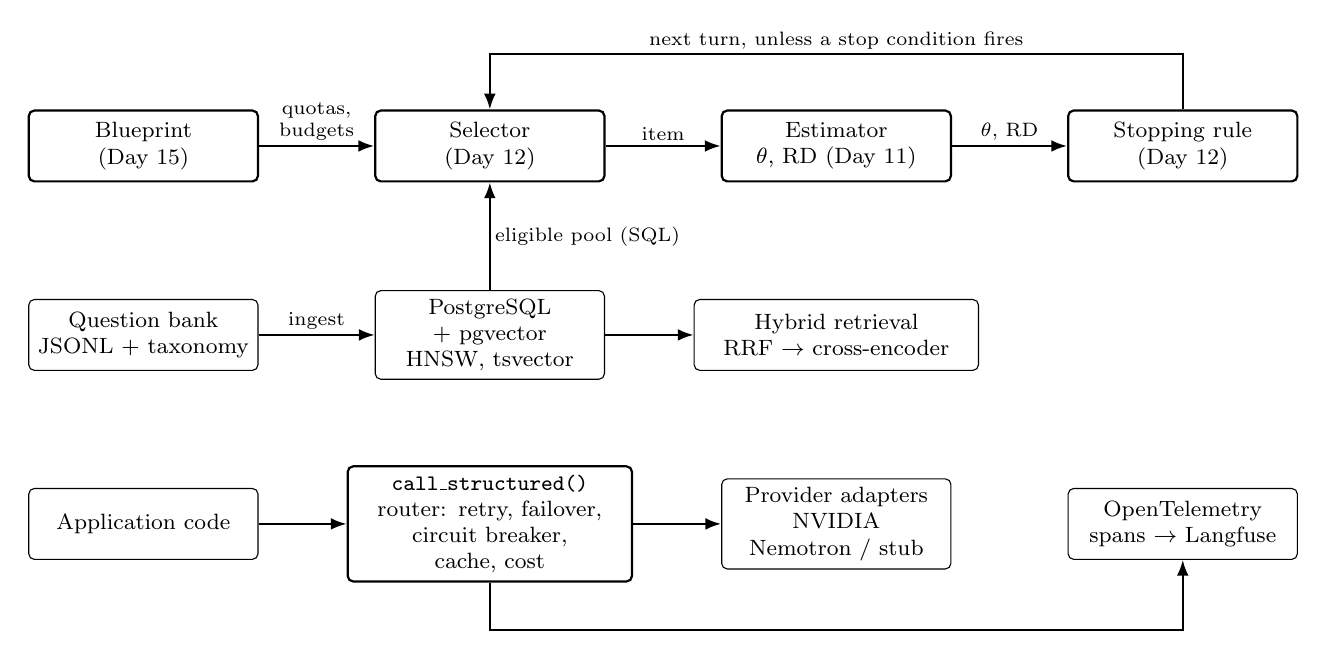
\begin{tikzpicture}[
  box/.style={draw, rounded corners=2pt, align=center, text width=27mm, minimum height=9mm, inner sep=3pt, font=\footnotesize},
  wide/.style={box, text width=34mm}, core/.style={box, thick},
  arrow/.style={-{Latex[length=2mm]}, thick}, lbl/.style={font=\scriptsize, align=center, inner sep=1.5pt, fill=white}]
  \node[core] (bp)   at (0,0)    {Blueprint\\(Day 15)};
  \node[core] (sel)  at (4.4,0)  {Selector\\(Day 12)};
  \node[core] (est)  at (8.8,0)  {Estimator\\ $\theta$, RD (Day 11)};
  \node[core] (stop) at (13.2,0) {Stopping rule\\(Day 12)};
  \draw[arrow] (bp)  -- node[lbl, above] {quotas,\\budgets} (sel);
  \draw[arrow] (sel) -- node[lbl, above] {item} (est);
  \draw[arrow] (est) -- node[lbl, above] {$\theta$, RD} (stop);
  \draw[arrow] (stop.north) -- ++(0,0.7) -| node[lbl, above, pos=0.25] {next turn, unless a stop condition fires} (sel.north);
  \node[box]  (bank) at (0,-2.4)   {Question bank\\JSONL + taxonomy};
  \node[box]  (pg)   at (4.4,-2.4) {PostgreSQL + pgvector\\HNSW, tsvector};
  \node[wide] (ret)  at (8.8,-2.4) {Hybrid retrieval\\RRF $\to$ cross-encoder};
  \draw[arrow] (bank) -- node[lbl, above] {ingest} (pg);
  \draw[arrow] (pg) -- (ret);
  \draw[arrow] (pg.north) -- node[lbl, right] {eligible pool (SQL)} (sel.south);
  \node[box]        (app)  at (0,-4.8)    {Application code};
  \node[wide,thick] (cs)   at (4.4,-4.8)  {\texttt{call\_structured()}\\router: retry, failover,\\circuit breaker, cache, cost};
  \node[box]        (prov) at (8.8,-4.8)  {Provider adapters\\NVIDIA Nemotron / stub};
  \node[box]        (obs)  at (13.2,-4.8) {OpenTelemetry\\spans $\to$ Langfuse};
  \draw[arrow] (app) -- (cs);
  \draw[arrow] (cs) -- (prov);
  \draw[arrow] (cs.south) -- ++(0,-0.6) -| (obs.south);
\end{tikzpicture}}
\caption{Architecture through Phase~3. Top: the adaptive loop. Middle: the Phase~2 data and retrieval layer. Bottom: the Phase~1 LLM chokepoint; no module outside \texttt{app/llm/} may call a provider. The grader that will connect the estimator to the chokepoint is Phase~4.}
\label{fig:architecture}
\end{figure}

\paragraph{The chokepoint.} Every model call goes through \texttt{call\_structured(task,
inputs, Schema)}, which returns a validated pydantic instance and a metadata record, or raises.
Below it sit a router (ordering, jittered retry, schema-repair retry, failover, a circuit
breaker, a cache, \texttt{Decimal} cost accounting) and provider adapters; the NVIDIA adapter is
the only file that knows the vendor exists, and the stub adapter replays recorded fixtures.
Structured output is negotiated -- strict \texttt{json\_schema}, then \texttt{json\_object}, then
prompt-only -- but pydantic validation is the guarantee and provider enforcement only an
optimisation. Structured calls are never streamed.

\paragraph{The adaptive loop.} The \emph{blueprint} answers ``what assessment do we need?'' and
never looks at an item; the \emph{selector} answers ``which question next?''; the
\emph{estimator} answers ``what do we believe?'' and is pure arithmetic with no I/O; the
\emph{stopping rule} answers ``should we end?''. Ability is stored at subtopic level only;
topic and domain values are computed on read so two sources of truth cannot drift.

\paragraph{Technical stack.} Python 3.12, FastAPI, pydantic v2, SQLAlchemy 2 (async), Alembic;
PostgreSQL with \texttt{pgvector} and native full-text search; Redis; NVIDIA
\texttt{nemotron-3.5-lightning-30b-a3b} via an OpenAI-compatible endpoint plus a deterministic stub;
\texttt{BAAI/bge-small-en-v1.5} (384-d) and \texttt{BAAI/bge-reranker-base} on CPU via fastembed
\cite{xiao2023cpack}; argon2id \cite{biryukov2016argon2}, 15-minute JWTs, 30-day single-use
rotating refresh tokens with reuse detection; structured JSON logging and OpenTelemetry with
three-layer redaction; Docker Compose and GitHub Actions.

\section{Data Design}
\label{sec:data-design}

Seven core tables have existed since Day~2 (Figure~\ref{fig:er}); a Day~8 migration added the
retrieval columns. Ability is canonical at the leaf (\texttt{skill\_states}, one row per user per
subtopic) and rolled up on read by precision-weighted aggregation. Session state will be a fold
over \texttt{interview\_events}, an append-only log; \texttt{turns} is the readable projection with a
client-supplied \texttt{turn\_id} for idempotency. The blueprint is serialised into
\texttt{interview\_sessions.blueprint} and re-validated on load, because a row is not a value this
process produced. \texttt{questions} carries both the dense vector and the generated
\texttt{tsvector} over the same \texttt{search\_document}, so the two retrievers can never index
different corpora.

\begin{figure}[htbp]
\centering
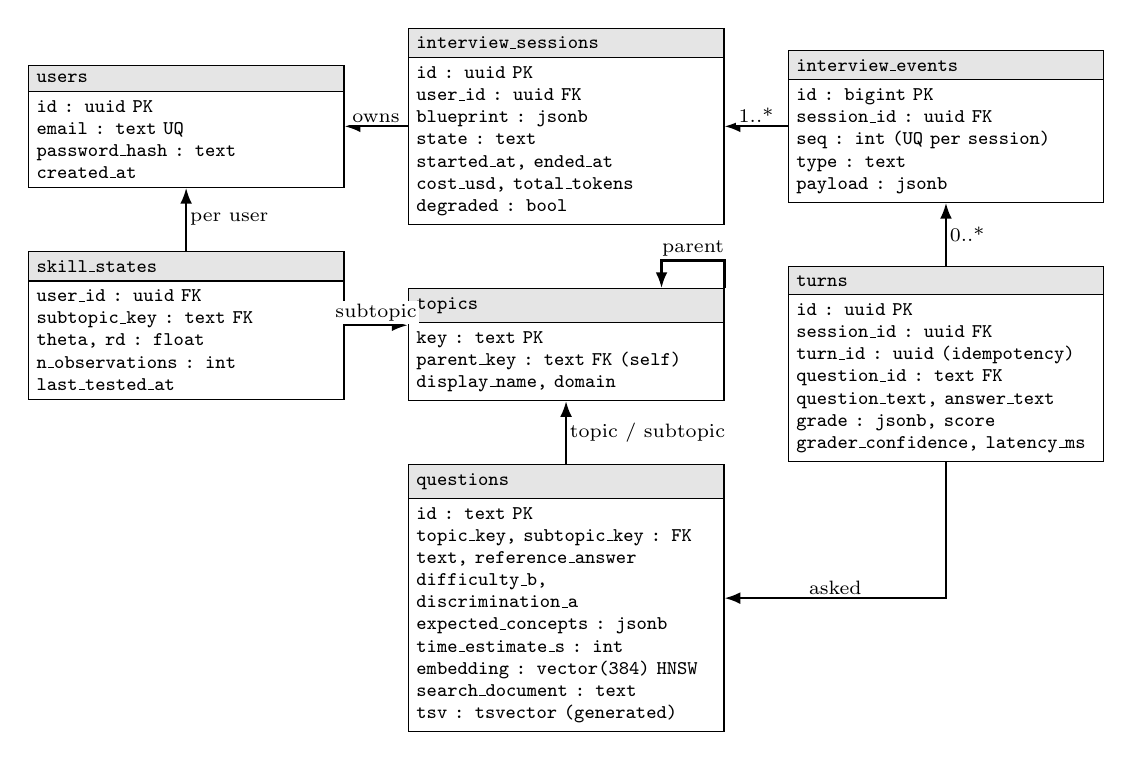
\begin{tikzpicture}[node distance=8mm and 8mm,
  ent/.style={draw, rectangle split, rectangle split parts=2, rectangle split part fill={black!10,white},
    font=\scriptsize\ttfamily, text width=38mm, inner sep=3pt, align=left},
  rel/.style={-{Latex[length=2mm]}, thick}, lbl/.style={font=\scriptsize, fill=white, inner sep=1pt}]
  \node[ent] (user) {\textbf{users}\nodepart{second} id : uuid PK\\ email : text UQ\\ password\_hash : text\\ created\_at};
  \node[ent, right=of user] (sess) {\textbf{interview\_sessions}\nodepart{second} id : uuid PK\\ user\_id : uuid FK\\ blueprint : jsonb\\ state : text\\ started\_at, ended\_at\\ cost\_usd, total\_tokens\\ degraded : bool};
  \node[ent, right=of sess] (event) {\textbf{interview\_events}\nodepart{second} id : bigint PK\\ session\_id : uuid FK\\ seq : int (UQ per session)\\ type : text\\ payload : jsonb};
  \node[ent, below=of user] (skill) {\textbf{skill\_states}\nodepart{second} user\_id : uuid FK\\ subtopic\_key : text FK\\ theta, rd : float\\ n\_observations : int\\ last\_tested\_at};
  \node[ent, below=of sess] (topic) {\textbf{topics}\nodepart{second} key : text PK\\ parent\_key : text FK (self)\\ display\_name, domain};
  \node[ent, below=of event] (turn) {\textbf{turns}\nodepart{second} id : uuid PK\\ session\_id : uuid FK\\ turn\_id : uuid (idempotency)\\ question\_id : text FK\\ question\_text, answer\_text\\ grade : jsonb, score\\ grader\_confidence, latency\_ms};
  \node[ent, below=of topic] (q) {\textbf{questions}\nodepart{second} id : text PK\\ topic\_key, subtopic\_key : FK\\ text, reference\_answer\\ difficulty\_b, discrimination\_a\\ expected\_concepts : jsonb\\ time\_estimate\_s : int\\ embedding : vector(384) HNSW\\ search\_document : text\\ tsv : tsvector (generated)};
  \draw[rel] (sess.west) -- node[lbl, above] {owns} (user.east);
  \draw[rel] (event.west) -- node[lbl, above] {1..*} (sess.east |- event.west);
  \draw[rel] (turn.north) -- node[lbl, right] {0..*} (event.south);
  \draw[rel] (skill.north) -- node[lbl, right] {per user} (user.south);
  \draw[rel] (skill.east) -- node[lbl, above] {subtopic} (topic.west |- skill.east);
  \draw[rel] (topic.north east) -- ++(0,0.35) -| node[lbl, above, pos=0.25] {parent} ([xshift=-8mm]topic.north east);
  \draw[rel] (q.north) -- node[lbl, right] {topic / subtopic} (topic.south);
  \draw[rel] (turn.south) |- node[lbl, above, pos=0.75] {asked} (q.east);
\end{tikzpicture}
\caption{Entity--relationship view of the seven core tables; arrows point from the referencing table to the referenced one.}
\label{fig:er}
\end{figure}

\section{Implementation Details}
\label{sec:impl}

About 19,000 lines under \texttt{backend/app/} are covered by 1,697 collected tests.

\subsection{Phase 1: Foundations and the LLM Chokepoint (Days 1--5)}

A multi-stage non-root Dockerfile and a health-checked Compose stack; \texttt{/healthz} touches
no dependency (failure means \emph{restart}) while \texttt{/readyz} probes PostgreSQL and Redis
under a deadline and reports whether a provider is in rotation without a model call (failure
means \emph{stop routing}); a \texttt{migrate} service runs \texttt{alembic upgrade head} before the
API starts. Authentication uses a cheap-to-verify access JWT and a single-use refresh token whose reuse is detectable and revokes the whole family; login is timing-equalised against a decoy hash. In the chokepoint, model reasoning is separated
from the answer inside the adapter and only its token count travels onward; tokens are summed
across every attempt including schema repairs; a \texttt{price\_known} flag makes an unlisted model
read as ``unknown cost'' rather than ``free''. Span attributes are a projection of the same
\texttt{CallMeta} record used for cost, so a trace and a cost report cannot disagree. A significant
finding was that \texttt{LOG\_LEVEL=DEBUG} made the OpenAI SDK log the full prompt (10,483
characters per call); HTTP libraries are now floored at INFO (1,732 characters, no content). The stub provider implements the same \texttt{LLMProvider} interface; fixtures are keyed by a hash of the whole request, and a replayed answer is labelled \texttt{stub\_replay} on the span, a label the data file cannot influence.

\subsection{Phase 2: Question Bank and Hybrid Retrieval (Days 6--10)}

The bank is a \texttt{taxonomy.json} (three domains, six topics, thirty-five subtopics) and one
JSONL file per domain. Each item carries $b\in[-3,3]$, $a$, three to six weighted expected
concepts, misconceptions, a reference answer, follow-up seeds, a time estimate and review
provenance; the schema uses \texttt{extra="forbid"} so a misspelt key cannot silently drop
\texttt{expected\_concepts}, and \texttt{reviewed} is not accepted without a named reviewer and date. A
bank-level validator collects every error, checks near-duplicates by 4-gram Jaccard and flags
concept keys one character apart. Sixty items pass with zero warnings.

Each question is embedded from one canonical \texttt{document\_text()} -- the question, humanised
concept keys, taxonomy path and tags, not the id, difficulty or reference answer -- stored as
\texttt{search\_document}, from which the \texttt{tsvector} is generated; this followed the discovery
that vector and lexical search had been indexing different corpora. Rows store the embedding
model id and a SHA-256 of the embedded text, so re-ingest does zero model work unless something
changed. Rankings are fused by reciprocal rank fusion \cite{cormack2009rrf},
\begin{equation}
  \mathrm{RRF}(d) = \sum_{r\in\{\text{vector},\,\text{lexical}\}} \frac{1}{k+\mathrm{rank}_r(d)}, \qquad k=60,
  \label{eq:rrf}
\end{equation}
using ranks only because cosine similarity and \texttt{ts\_rank\_cd} live on unrelated scales.
The HNSW index is present but correctly unused by the planner at 60 rows; a test forces it to
prove compatibility. The optional cross-encoder \cite{nogueira2019bert} reads the same
\texttt{search\_document}, emits an unbounded logit that is never turned into a pseudo-probability,
and falls back to stage-one order with \texttt{reranked=False} if the model fails to load. Forty
labelled queries (graded 0--2, written before any retrieval ran, each tagged by \emph{kind}) drive
Recall@K, MRR and nDCG@10 \cite{jarvelin2002ndcg}, all tested against hand-worked values.

\subsection{Phase 3: The Adaptive Engine (Days 11--15)}
\label{sec:engine}

\paragraph{Ability model (Day 11).} \texttt{app/ability.py} imports \texttt{math},
\texttt{collections.abc} and \texttt{dataclasses} and nothing else. The per-subtopic state is a frozen
$\mathrm{AbilityState}(\theta,\mathrm{RD},n)$ with $\theta\in[-3,3]$, $\mathrm{RD}\in[0.30,1.30]$ and
cold-start prior $\theta=0$, $\mathrm{RD}=1.30$. Prediction is the 2PL model \cite{lord1980irt},
\begin{equation}
  p(\theta,b) = \frac{1}{1+e^{-a(\theta-b)}},
  \label{eq:2pl}
\end{equation}
with a two-branch numerically stable sigmoid. The update is an Elo-style step
\cite{elo1978rating}, exactly one gradient step on the log loss,
\begin{equation}
  \Delta\theta = K\,(s-p), \qquad \theta_{\text{new}} = \theta + \operatorname{clip}(\Delta\theta,\pm0.5),
  \qquad K = K_0\, f_{\text{conf}}\, f_{\text{rd}}\, f_{\text{stake}},
  \label{eq:update}
\end{equation}
with $K_0=0.6$, $f_{\text{rd}}=\min(1.6,\mathrm{RD}/0.6)$, $f_{\text{conf}}$ the grader's confidence
and $f_{\text{stake}}\in\{1.0,0.5\}$ for bank versus generated items. Discrimination $a$ shapes $p$
and the uncertainty but is deliberately not a factor of $K$. The score $s\in[0,1]$ is validated,
never clamped. Uncertainty follows Glicko \cite{glickman1999glicko},
\begin{equation}
  \mathrm{RD}_{\text{new}} = \big(1/\mathrm{RD}^2 + a^2\,p\,(1-p)\big)^{-1/2},
  \label{eq:rd}
\end{equation}
which only decreases within a session. Aggregation is precision-weighted, $w_i=1/\mathrm{RD}_i^2$:
\begin{equation}
  \theta_{\text{parent}} = \frac{\sum_i w_i\theta_i}{\sum_i w_i}, \qquad
  \mathrm{RD}_{\text{parent}} = \Big(\sum_i w_i\Big)^{-1/2}.
  \label{eq:rollup}
\end{equation}
Children $(1.0,0.2)$ and $(0.0,1.0)$ give $\theta=0.9615$, not the plain average $0.5$, because
the first was measured 25 times more precisely. The plan's worked example is reproduced by a
test: from $\theta=0.30$, $\mathrm{RD}=0.90$, $b=0.80$, score $0.70$, confidence $0.85$, the model
predicts $p=0.3775$, applies $K=0.765$, moves $\theta$ by $+0.247$ to $0.547$ and tightens RD to
$0.825$.

\paragraph{Item selection (Day 12).} Selection is three stages so each can be tested and
explained alone. \emph{Hard constraints are filters, not penalties}, run as SQL with bound
parameters: not asked, topic quota left, $|b-\theta_{\text{subtopic}}|\le1.5$, fits the remaining
clock. The same rule exists as a Python predicate, \texttt{ineligibility\_reason()}, and an
integration test asserts both select identical rows over the real bank; a unit test asserts a
key containing \texttt{'; DROP TABLE questions; --} appears only in bound parameters. The objective
uses normalised Fisher information $p(1-p)/0.25$ without $a^2$, so a sharp item cannot silently
receive four times the information term:
\begin{equation}
\begin{aligned}
  \mathrm{score}(q) = {}& 0.40\,\tfrac{p(1-p)}{0.25} + 0.25\,\mathrm{jd\_weight}[\mathrm{topic}(q)]
    + 0.15\,\mathrm{resume\_affinity}(q) \\
  &+ 0.15\,\mathrm{coverage\_deficit}(\mathrm{topic}(q)) - 0.10\,\mathrm{redundancy}(q)
    - 0.05\,\tfrac{\mathrm{time\_estimate}(q)}{\mathrm{time\_left}},
\end{aligned}
\label{eq:objective}
\end{equation}
where redundancy is the maximum cosine similarity to any asked item (Phase~2 vectors; nothing
is embedded at selection time). The weights are documented design choices, not measured optima.
\emph{$\varepsilon$-greedy}: with probability 0.90 the argmax, otherwise a uniform draw over the
top five, with exactly one random draw per selection so a seeded session is reproducible; a
pure argmax would be memorisable and would never collect the off-policy data needed to correct
a mis-authored $b$. \emph{Stopping} fires on any of: RD $<0.40$ for every required topic
(through Eq.~\eqref{eq:rollup}); items $\ge$ budget; time $\ge$ budget; three consecutive
$|\Delta\theta|<0.05$. Every reason that fired is reported.

\paragraph{Simulation (Day 13).} A test can show \texttt{score\_item} computes
Eq.~\eqref{eq:objective}; it cannot show that asking in that order measures a candidate better.
The simulation package is that evidence and runs with zero tokens, no database and no network.
The committed 60-item bank is a poor laboratory (a 20-item session consumes a third of it;
subtopics hold 1--3 items; every $a$ is 1.0), so the simulator generates 192 items over three
topics $\times$ two subtopics with $b$ spread over $[-2.5,2.5]$, $a\in[0.7,1.6]$ and 16-d
embeddings whose geometry is asserted. Two hundred candidates receive hidden abilities drawn
hierarchically. Observed scores are $s\sim\mathrm{Beta}(p\kappa,(1-p)\kappa)$, $\kappa=10$ -- mean
$p$, standard deviation 0.151 on a coin-flip item, roughly two competent graders' disagreement.
Ground truth is structurally unreachable: a strategy's arguments are (state, bank, rng) and no
field references a candidate. \emph{Adaptive} calls the shipped \texttt{choose\_next};
\emph{random} calls the same \texttt{filter\_eligible} and draws uniformly, so their contrast
isolates the ranking objective; \emph{fixed} walks an easy-to-hard paper and cannot apply the
difficulty window, so that contrast bundles two mechanisms. The response generator is keyed by
(candidate, item) so every policy sees the same answer to the same question; seeds derive
through BLAKE2b; the whole experiment is byte-identical across runs, asserted by test. An
ablation reruns adaptive six times with one weight zeroed each time.

\paragraph{Convergence analysis (Day 14).} Each session records a \texttt{TrajectoryStep} per
turn -- belief about every subtopic, the item, score, $\Delta\theta$ and error against hidden
truth -- written after the update from state the policy already had; Day~13's report
regenerates byte-identically, proving this is an observation not a change. Curves forward-fill
stopped sessions. Ten figures are written as deterministic SVG by a committed script.

\paragraph{Blueprint builder (Day 15).} \texttt{AssessmentSpec} is the possibly under-specified
\emph{request} (role, level, mode, duration, weighted topics); \texttt{Blueprint} is the fully
determined \emph{contract}; \texttt{build\_blueprint} is the only place they meet, and two adapters
hand Day~12 exactly the arguments it declared. \texttt{app.selection} does not import
\texttt{app.blueprint}; a test asserts it. Quotas are allocated by largest remainder with per-topic
floors and caps (flooring starves the smallest share; rounding overspends). Seconds-per-item
per mode come from the committed bank's quartiles (screening 300, standard 330, deep-dive
390\,s); seniority maps to a cold-start $\theta$ (junior $-0.5$ $\ldots$ staff $+1.0$) and never
reduces RD. Twenty-four validation rules run in \texttt{\_\_post\_init\_\_} so an invalid blueprint
cannot exist; it serialises to JSON for the session row and re-validates on load.

% =====================================================================
\chapter{Results and Evaluation}
\label{ch:results}

\section{Testing Methodology}

1,697 tests are collected (Table~\ref{tab:tests}); the default offline suite runs in about 18
seconds with no network, database, model or key. Numerical modules are tested against
hand-worked values, and property tests sweep deterministic grids (about 8,100 update
combinations; every subset of a seven-element aggregation pool) so a failure is identical on
every machine. 138 integration tests run against real PostgreSQL and Redis (migrations, auth,
ingest idempotency, hybrid retrieval, SQL/predicate equivalence of the selection constraints)
and skip with an actionable message when the stack is down. 22 model tests and one live smoke
test are opt-in. No load test and no user test has been run; every Phase~3 result is from
simulation. \texttt{ruff}, \texttt{mypy --strict} and gitleaks are clean. \emph{No test asserts that
any policy beats another}: that is an empirical hypothesis, not a software invariant.

\begin{table}[htbp]
\centering\small
\begin{tabular}{lrl@{\qquad}lrl}
  \toprule
  \textbf{Package} & \textbf{Tests} & \textbf{Ph.} & \textbf{Package} & \textbf{Tests} & \textbf{Ph.} \\
  \midrule
  \texttt{unit/simulation} & 323 & 3 & \texttt{unit/obs} & 100 & 1 \\
  \texttt{unit/llm} & 267 & 1 & \texttt{unit/test\_ability.py} & 97 & 3 \\
  \texttt{unit/selection} & 235 & 3 & \texttt{unit/evaluation} & 75 & 2 \\
  \texttt{unit/blueprint} & 226 & 3 & \texttt{unit/bank} & 49 & 2 \\
  \texttt{unit/retrieval} & 122 & 2 & other unit; \texttt{integration/*}; smoke & 64; 138; 1 & 1--3 \\
  \bottomrule
\end{tabular}
\caption{Test distribution at the close of Phase~3 (1,697 collected; default run 1,536 passed, 138 skipped, 23 deselected).}
\label{tab:tests}
\end{table}

\section{Phase 1: Live Verification of the Chokepoint}
\label{sec:live-verification}

The exit-gate probe ran against the live NVIDIA endpoint: strict \texttt{json\_schema} accepted;
328 input and 23 output tokens; zero reasoning tokens; zero schema retries; 1,265\,ms; cost
\$0.000000 with \texttt{price\_known=True}. Failure paths were verified live: an invalid key raises
\texttt{ProviderAuthError} without the key in the message; a dead primary is answered with
\texttt{failover\_count=1}; a 1\,ms deadline raises \texttt{AllProvidersFailedError}. A DEBUG log capture
of 5,615 characters contained neither the key nor \texttt{nvapi}. A real span was read back from a
self-hosted Langfuse with model and token counts and without prompt or answer.

\section{Phase 2: Retrieval Ablation}
\label{sec:retrieval-results}

\begin{table}[htbp]
\centering\small
\begin{tabular}{lrrrrr}
  \toprule
  \textbf{Method} & \textbf{Recall@5} & \textbf{Recall@10} & \textbf{MRR} & \textbf{nDCG@10} & \textbf{ms/query} \\
  \midrule
  Vector only & 0.850 & 0.883 & 0.908 & 0.877 & 65.5 \\
  Lexical only & 0.208 & 0.208 & 0.300 & 0.269 & 1.1 \\
  \textbf{Hybrid RRF} & \textbf{0.850} & \textbf{0.883} & \textbf{0.921} & \textbf{0.886} & 58.4 \\
  Hybrid + reranker & 0.746 & 0.875 & 0.906 & 0.858 & 3448.0 \\
  \bottomrule
\end{tabular}
\caption{Retrieval ablation (Day 10): 40 labelled queries, 60 items, real models. Hybrid RRF is best on every metric; the cross-encoder made every metric worse at 42$\times$ the latency.}
\label{tab:retrieval}
\end{table}

The result (Table~\ref{tab:retrieval}) was not the expected one and was investigated rather than
tuned away. By query kind, the reranker is perfect on exact-term queries (MRR 1.000 vs hybrid
0.944 on 9 lexical queries) but worst on the three queries written to reward it (0.778 vs
1.000). The mechanism is visible per query: hybrid already places the correct answer at rank~1
for 34 of 40 queries, so there is almost nothing left to win, and the cross-encoder reorders
candidates it finds near-equivalent. The hypothesis that showing it the full
\texttt{search\_document} was the cause was tested and rejected (full document MRR 0.906 versus bare
question 0.832). Nothing was changed. Latency: about 33\,ms of a hybrid query is embedding the
query and about 3\,ms is both SQL queries; the cross-encoder costs about 100\,ms per candidate on
150--200-token documents, so 40 candidates is about 4\,s against a plan estimate of 250\,ms --
document length, not the model.

\section{Phase 3: Policy Comparison in Simulation}
\label{sec:policy-results}

Table~\ref{tab:policies} is the main result: 200 candidates, a 20-item budget, quotas $\{8,7,5\}$
from JD weights $\{0.9,0.7,0.5\}$, seed 20260101. MAE is over every blueprint subtopic with
unmeasured ones left at the prior -- the number a report would print; MAE(seen) covers only
subtopics a policy asked about.

\begin{table}[htbp]
\centering\small
\begin{tabular}{lrrrrrrr}
  \toprule
  \textbf{Policy} & \textbf{MAE} & \textbf{RMSE} & \textbf{MAE(seen)} & \textbf{Subtopics/6} & \textbf{Items} & $\mathbf{|b-\theta|}$ & \textbf{Coverage} \\
  \midrule
  Adaptive & 0.433 & 0.538 & \textbf{0.333} & 4.71 & 18.9 & \textbf{0.136} & 86.0\% \\
  Random & \textbf{0.422} & \textbf{0.504} & 0.415 & \textbf{5.84} & 19.0 & 0.756 & \textbf{87.0\%} \\
  Fixed & 0.495 & 0.575 & 0.494 & 5.50 & \textbf{16.6} & 1.305 & 69.5\% \\
  \bottomrule
\end{tabular}
\caption{Policy comparison at a 20-item budget (Day 13). $|b-\theta|$ is the mean gap between item difficulty and the running estimate at selection time. No policy wins every column.}
\label{tab:policies}
\end{table}

\textbf{The precise conclusion.} Adaptive selection substantially improves precision on the
subtopics it investigates (MAE(seen) 0.333 against 0.415 and 0.494) and its difficulty matching
(0.136 against 0.756 and 1.305), on an identical eligibility pool. In this synthetic environment
it sacrifices enough breadth (4.71 of 6 subtopics against 5.84) that \textbf{random selection
edges it on overall MAE, 0.422 to 0.433}. Against the fixed paper adaptive wins on error,
difficulty matching and coverage but that comparison is uncontrolled. The between-candidate
interquartile range of final MAE is about 0.24 for every policy -- twenty times the 0.011 gap.
No hypothesis test was run and no significance is claimed in either direction.

\paragraph{Weight ablation.} Removing the information term is the largest degradation
(MAE $+0.039$; the difficulty gap rises from 0.136 to 0.802). Removing redundancy drops coverage
from 4.71 to 4.11 subtopics -- similarity is highest within a subtopic, so the penalty was doing
coverage work. Removing coverage, time or JD costs $+0.010$, $+0.009$ and $+0.008$. Removing the
\emph{resume} term is the only improvement and the largest single effect ($-0.058$, coverage
5.99 of 6): with it on, 59.9\% of items land on the two resume-mentioned subtopics against a
uniform 33.3\%, because the coverage term is topic-level while $\theta$ is subtopic-level, and
resume affinity is the only always-on subtopic-level term. \textbf{This is a diagnostic
finding, not a recommendation}: the synthetic resume carries no ability signal by construction,
so the experiment can measure the term's cost but not its benefit. The weight stays at 0.15.

\section{Phase 3: Convergence and Trajectories}
\label{sec:convergence-results}

Figure~\ref{fig:mae-curve} shows the population-mean MAE after each question. Day~13's endpoint
is not a shape: \textbf{adaptive is ahead for the first eight questions and behind from the
ninth}. Coverage explains why: the policies are level for three questions, and by question~8
random has touched one whole subtopic more (4.63 against 3.63), widening to 1.13 at the budget.
An untouched subtopic contributes its whole prior error, so adaptive's depth advantage is real,
bounded, and spent after eight questions -- a fact about the budget as much as the policy. Among
sessions that reached all six subtopics, adaptive's MAE is 0.339 (46 sessions) against random's
0.425 (179) -- an association, not a cause, since the bin selects on what the policy did.

\begin{figure}[htbp]
\centering
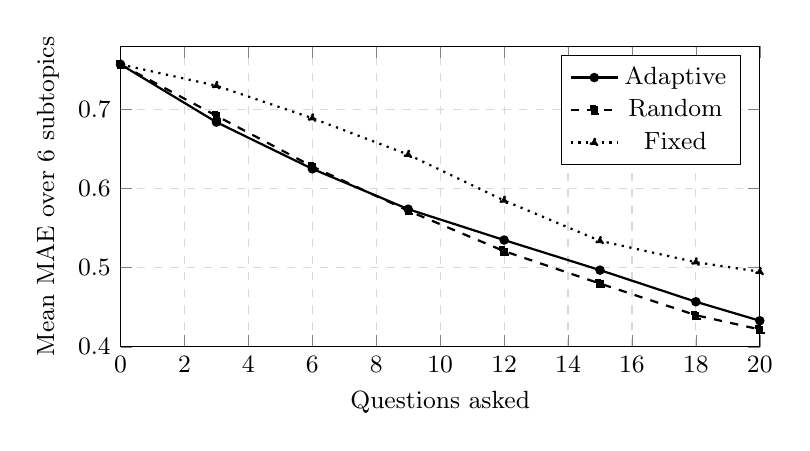
\begin{tikzpicture}
\begin{axis}[width=0.8\linewidth, height=5.4cm, xlabel={Questions asked}, ylabel={Mean MAE over 6 subtopics},
  xmin=0, xmax=20, ymin=0.40, ymax=0.78, grid=major, grid style={dashed, gray!30},
  legend pos=north east, legend style={font=\small}, tick label style={font=\small}, label style={font=\small}]
\addplot[thick, mark=*, mark size=1.3pt] coordinates {(0,0.757)(3,0.684)(6,0.625)(9,0.574)(12,0.535)(15,0.497)(18,0.457)(20,0.433)};
\addlegendentry{Adaptive}
\addplot[thick, dashed, mark=square*, mark size=1.3pt] coordinates {(0,0.757)(3,0.692)(6,0.628)(9,0.572)(12,0.521)(15,0.480)(18,0.440)(20,0.422)};
\addlegendentry{Random}
\addplot[thick, dotted, mark=triangle*, mark size=1.6pt] coordinates {(0,0.757)(3,0.730)(6,0.689)(9,0.643)(12,0.585)(15,0.534)(18,0.507)(20,0.495)};
\addlegendentry{Fixed}
\end{axis}
\end{tikzpicture}
\caption{Mean MAE against questions asked (Day 14, seed 20260101, 200 candidates). Adaptive leads random through question~8 and trails from question~9. Redrawn from the committed table; the original is \texttt{evals/reports/convergence/mae-vs-questions.svg}.}
\label{fig:mae-curve}
\end{figure}

\paragraph{Convergence criteria and stopping.} Neither criterion separates the policies:
adaptive reaches MAE $\le0.5$ in 6.4 items (149 of 200 sessions) against random's 6.1 (152);
\emph{no} policy reaches worst-topic RD $\le0.35$ in any of 600 sessions at 20 or 60 items, and
the stopping rule's RD $<0.40$ fires in two adaptive sessions of 200 at 60 items. The arithmetic
explains it: an informative answer adds about 0.33 of precision, a two-subtopic topic starts at
1.18 and needs 6.25 to reach RD $<0.40$ -- about 45 items for a three-topic blueprint. Either the
threshold is tighter than a 20-item interview can earn or the interview is thinner than the
threshold assumes; the evidence cannot separate these and the constant was not moved. Sessions
stopped on the item budget (172 adaptive, 174 random, 139 fixed) or on
\texttt{no\_new\_information} (28, 26, 61); 29 of the 61 fixed sessions stopped at question~3, the
earliest possible, because an easy-first paper opens with answers the cold-start model predicts
confidently. Reversal rates of 32--36\% (against $\sim$50\% for an estimate sitting on the truth)
show every policy's estimate is still travelling when the interview ends. \textbf{The Phase~3 gate
``adaptive reaches a given precision in materially fewer items than random'' is not met.}

\paragraph{The blueprint and the pacing finding.} 226 tests include an end-to-end class that
walks a whole session driven by a blueprint, asserting no quota exceeded, no repeat, the clock
never overspent, and a stored-and-reloaded blueprint runs the identical session. Deriving the
item budget from the committed bank produced a number worth stating plainly: \textbf{a
45-minute standard assessment fits 8 questions, not 20} (median item 330\,s against the
simulation's 135\,s). Day~14 measured the crossover at question~9, so adaptive was ahead for
the whole length of a real assessment -- a suggestive alignment between two worlds, recorded as
the next experiment, not as a result. Writing the tests also found that a Day~13 docstring
claimed quotas $\{9,7,4\}$ where the code has always produced $\{8,7,5\}$; a docstring was wrong,
not a behaviour.

\section{Analysis}
\label{sec:gates}

\begin{table}[htbp]
\centering\small
\begin{tabularx}{\linewidth}{L{0.04\linewidth} Y L{0.4\linewidth}}
  \toprule
  \textbf{Ph.} & \textbf{Gate} & \textbf{Status} \\
  \midrule
  1 & \texttt{docker compose up} from a clean clone gives a working API & Met \\
  1 & Register $\to$ login $\to$ authenticated \texttt{/me} & Met \\
  1 & One LLM call through \texttt{call\_structured()} in tracing with cost & Met (verified live) \\
  1 & Dead primary provider fails over, proven by a test & Met (unit and live) \\
  1 & CI is green on a PR & Green locally; not yet run on GitHub (nothing pushed before Day~30 by rule) \\
  \midrule
  2 & 150 reviewed items passing CI validation & Partial: 60 items, validated, none human-reviewed \\
  2 & \texttt{GET /questions/search} in $<300$\,ms & Endpoint not built; retrieval layer answers in $\sim$58\,ms via a script \\
  2 & Four-row ablation table & Met; hybrid RRF won, reranker did not \\
  \midrule
  3 & \texttt{test\_ability.py} passes including property tests & Met (97 tests) \\
  3 & Convergence chart from a committed script & Met (ten deterministic figures) \\
  3 & Adaptive reaches a given precision in materially fewer items than random & \textbf{Not met}; recorded, not redefined \\
  \bottomrule
\end{tabularx}
\caption{Phase exit gates through Day 15.}
\label{tab:gatestab}
\end{table}

\paragraph{Where expectations were exceeded.} The offline discipline: every default test and the
project's central evidence run without a network, database, model or key, cost zero tokens and
reproduce byte-for-byte. The structured-output ladder, built defensively before a key existed,
was accepted at the strongest rung live, making the step-down a free safety net. Redaction was
verified against real log output rather than assumed.

\paragraph{Challenges and resolution.} \emph{Verification found defects tests had not}: a
migration wiped the logging configuration (Alembic's \texttt{fileConfig}); the fixture recorder
filed a repaired answer under an unreachable key; a fixture could impersonate a live call; two
retrievers indexed different corpora; DEBUG logging recorded prompts. Each has a regression test
confirmed to fail when reintroduced. \emph{The reranker did not win}; the result was broken down
by kind, a hypothesis tested and rejected, and no default changed. \emph{Adaptive did not beat
random on overall error}; the trajectory located the mechanism, the ablation the term, the
blueprint the budget mismatch, and none was used to retune anything, because fitting the system
to one synthetic experiment is fitting the experiment. \emph{Phase~2 slipped}: 90 items and the
endpoint were not built; the gate is recorded as partial.

% =====================================================================
\chapter{Conclusion}
\label{ch:conclusion}

\section{Summary of Work}

Fifteen of forty-five days are complete. Phase~1 delivered a production-shaped service: a
containerised FastAPI application with migrations, two-token authentication with rotation and
reuse detection, a single validated and cost-accounted door for every LLM call with retry,
failover and a circuit breaker, structured logging and tracing with redaction, CI, and an
offline provider replaying real recorded answers. Phase~2 delivered a validated 60-item bank
over a 35-subtopic taxonomy, embedding and lexical indexing, hybrid retrieval by reciprocal rank
fusion, an optional reranker and a measured four-row ablation. Phase~3 delivered the adaptive
engine: a pure-arithmetic ability model, a three-stage selector with SQL-enforced constraints,
a six-term objective with $\varepsilon$-greedy exploration, a four-condition stopping rule, a
zero-token simulation of 200 candidates under three policies with a seven-way ablation, a
per-turn convergence analysis, and a validated, serialisable blueprint that closes the loop from
requirements to stopping. Objective~1 is met, Objective~2 partially, Objective~3 on two of three
gates; the third is not met and the evidence has been presented in full rather than adjusted.

\section{Key Findings and Limitations}

\begin{enumerate}
  \item \textbf{Retrieval (validated):} hybrid RRF is the best configuration on 40 queries over
    60 documents (MRR 0.921, $\sim$58\,ms); the cross-encoder lowered every metric at 42$\times$
    the latency, most plausibly because a tiny corpus leaves nothing to win -- not a verdict on
    reranking at scale.
  \item \textbf{Adaptive vs random (validated):} adaptive is materially more precise on what it
    measures (0.333 vs 0.415) and matches difficulty far better (0.136 vs 0.756), covers fewer
    subtopics, and \textbf{random has slightly lower overall MAE (0.422 vs 0.433)} at 20 items.
    Adaptive was not shown superior overall; no significance is claimed either way.
  \item \textbf{Mechanism (validated):} the adaptive lead is spent, not absent -- ahead through
    question~8, behind from question~9, because random has measured one more subtopic.
  \item \textbf{Ablation (validated):} the information term is the one weight the experiment
    positively supports; the resume term concentrates 59.9\% of items on two subtopics and hurts
    accuracy here, but the experiment can measure only its cost, so it stays.
  \item \textbf{Calibration (validated):} the precision stopping condition fires in 0 of 600
    sessions at 20 items; roughly 45 items would be needed; threshold versus budget cannot be
    decided from this evidence.
  \item \textbf{Pacing (unexpected):} a real 45-minute assessment holds 8 questions, one short
    of the measured crossover -- the obvious next experiment.
  \item \textbf{Engineering:} the highest-value defects were found by running the system, not by
    the tests that preceded the run; each now has a regression test.
\end{enumerate}

\paragraph{Limitations.} Every Phase~3 number describes one synthetic environment at one seed:
six subtopics, a 192-item bank, candidates who answer exactly the 2PL model with Beta noise, a
resume with no signal. No real candidate, question or interview has been measured; no
statistical test was run; the adaptive-vs-fixed comparison bundles mechanisms; the coverage
bins are observational. The evaluation set is 40 queries from a single annotator with no
confidence intervals. The bank holds 60 of 150 items, none human-reviewed, with a thin concept
vocabulary and a difficulty distribution that leans hard (49 of 60 at $b\ge0$).

\section{Future Work and Recommendations}
\label{sec:future}

\begin{enumerate}
  \item \textbf{Grader and scoring pipeline (Phase~4):} concept-coverage classification with
    evidence spans through the chokepoint, validated at QWK $\ge0.65$ on 120 labelled answers;
    length-, position- and jargon-bias probes; an injection suite targeting 0\% attack success;
    a CI guard on agreement. This turns the estimator's score input from a Beta draw into a
    measurement and is the precondition for any claim about real candidates.
  \item \textbf{Session orchestration (Phase~5):} the FSM, event log and public API; resume and
    JD parsing to derive the weights a blueprint currently takes as numbers.
  \item \textbf{Completing Phase~2:} ninety more items targeting $b<-0.5$; human review; the
    search endpoint; re-measuring the reranker on a larger corpus.
  \item \textbf{Re-run the simulation at realistic budgets} (8 and 12 items, bank-calibrated
    pacing) and \textbf{test significance across paired seeds}, so the crossover and the pacing
    finding are measured in the same world.
  \item \textbf{A subtopic-level coverage term}, measured in a controlled design before it is
    adopted, and a decision on \textbf{threshold versus budget} once real response data exist.
  \item \textbf{Deployment (Phase~6):} nothing before Day~30 by design; the
    \texttt{SameSite=Strict} cookie policy must be revisited once the front-end origin is known.
\end{enumerate}

\section{Final Remarks}

The project's thesis is that an interview policy should be a measurement algorithm rather than
a prompt. Fifteen days in, the algorithm exists, is pure enough to be tested exhaustively
offline, and has been put through the one experiment that could have embarrassed it. The
experiment did not confirm the strongest claim the plan hoped for; in a synthetic world adaptive
selection buys precision on what it measures rather than speed to a loose threshold. That
result is reported at full strength, and no weight, threshold or stopping constant was moved to
make the sentence read differently. Every result here regenerates byte-for-byte from a committed
script, every claim traces to a test or a table, and every gap between plan and build is written
down. That property is what will make the grader in Phase~4, and the real interviews after it,
measure something.

% =====================================================================
\chapter{System Modelling in UML}
\label{ch:uml}

This chapter models the system in three standard UML views \cite{booch2005uml}. Every class,
attribute and operation shown exists under \texttt{backend/app/} with the name given; use cases
belonging to later phases are drawn dashed.

\section{Use Case Diagram and Scenarios}

Figure~\ref{fig:usecase} shows four human actors and one external system. The
\emph{Candidate} takes interviews and reads reports; the \emph{Assessment Author} (a mentor, TA or
the candidate) defines what an assessment covers; the \emph{Bank Author} writes and reviews
items; the \emph{Developer} runs experiments and records fixtures; the \emph{LLM Provider} is
called, never calling.

\begin{figure}[htbp]
\centering
\resizebox{0.78\linewidth}{!}{%
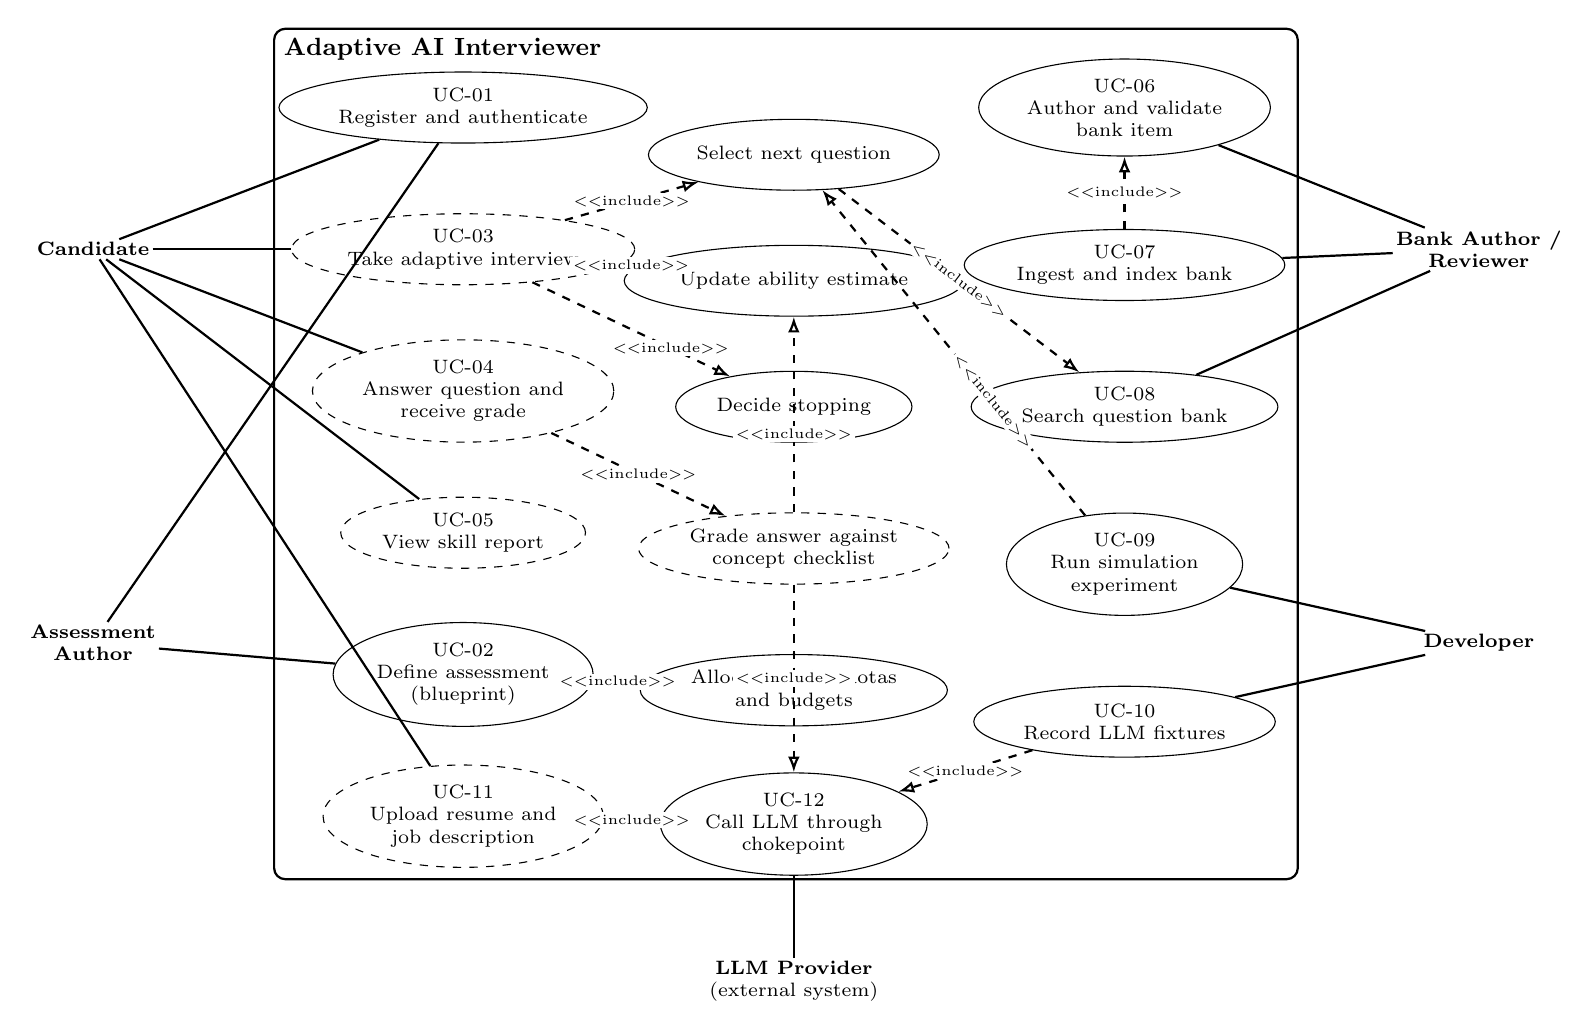
\begin{tikzpicture}[every node/.style={font=\scriptsize},
  uc/.style={usecase, minimum width=30mm}, ucp/.style={usecase, minimum width=30mm, dashed},
  ln/.style={thick}, inc/.style={-{Latex[open,length=2mm]}, dashed, thick}, inclbl/.style={font=\tiny, fill=white, inner sep=1pt}]
  \draw[thick, rounded corners=4pt] (-0.6,-9.6) rectangle (12.4,1.2);
  \node[anchor=north west, font=\small\bfseries] at (-0.6,1.2) {Adaptive AI Interviewer};
  \node[actor] (cand) at (-2.9,-1.6) {\textbf{Candidate}};
  \node[actor] (auth) at (-2.9,-6.6) {\textbf{Assessment}\\\textbf{Author}};
  \node[actor] (bank) at (14.7,-1.6) {\textbf{Bank Author /}\\\textbf{Reviewer}};
  \node[actor] (dev)  at (14.7,-6.6) {\textbf{Developer}};
  \node[actor] (llm)  at (6.0,-10.9) {\textbf{LLM Provider}\\(external system)};
  \node[uc]  (uc1) at (1.8,0.2)   {UC-01\\Register and authenticate};
  \node[ucp] (uc3) at (1.8,-1.6)  {UC-03\\Take adaptive interview};
  \node[ucp] (uc4) at (1.8,-3.4)  {UC-04\\Answer question and\\receive grade};
  \node[ucp] (uc5) at (1.8,-5.2)  {UC-05\\View skill report};
  \node[uc]  (uc2) at (1.8,-7.0)  {UC-02\\Define assessment\\(blueprint)};
  \node[ucp] (uc11) at (1.8,-8.8) {UC-11\\Upload resume and\\job description};
  \node[uc] (uc3a) at (6.0,-0.4)  {Select next question};
  \node[uc] (uc3b) at (6.0,-2.0)  {Update ability estimate};
  \node[uc] (uc3c) at (6.0,-3.6)  {Decide stopping};
  \node[ucp] (uc4a) at (6.0,-5.4) {Grade answer against\\concept checklist};
  \node[uc] (uc2a) at (6.0,-7.2)  {Allocate topic quotas\\and budgets};
  \node[uc] (uc12) at (6.0,-8.9)  {UC-12\\Call LLM through\\chokepoint};
  \node[uc] (uc6) at (10.2,0.2)   {UC-06\\Author and validate\\bank item};
  \node[uc] (uc7) at (10.2,-1.8)  {UC-07\\Ingest and index bank};
  \node[uc] (uc8) at (10.2,-3.6)  {UC-08\\Search question bank};
  \node[uc] (uc9) at (10.2,-5.6)  {UC-09\\Run simulation\\experiment};
  \node[uc] (uc10) at (10.2,-7.6) {UC-10\\Record LLM fixtures};
  \foreach \a/\u in {cand/uc1,cand/uc3,cand/uc4,cand/uc5,cand/uc11,auth/uc2,auth/uc1,bank/uc6,bank/uc7,bank/uc8,dev/uc9,dev/uc10,llm/uc12} \draw[ln] (\a) -- (\u);
  \draw[inc] (uc3) -- node[inclbl] {<<include>>} (uc3a);
  \draw[inc] (uc3) -- node[inclbl, pos=0.6] {<<include>>} (uc3b);
  \draw[inc] (uc3) -- node[inclbl, pos=0.7] {<<include>>} (uc3c);
  \draw[inc] (uc4) -- node[inclbl] {<<include>>} (uc4a);
  \draw[inc] (uc4a) -- node[inclbl, pos=0.4] {<<include>>} (uc3b);
  \draw[inc] (uc2) -- node[inclbl] {<<include>>} (uc2a);
  \draw[inc] (uc4a) -- node[inclbl, pos=0.5] {<<include>>} (uc12);
  \draw[inc] (uc11) -- node[inclbl, pos=0.5] {<<include>>} (uc12);
  \draw[inc] (uc10) -- node[inclbl, pos=0.5] {<<include>>} (uc12);
  \draw[inc] (uc3a) -- node[inclbl, pos=0.5, sloped] {<<include>>} (uc8);
  \draw[inc] (uc9) -- node[inclbl, pos=0.35, sloped] {<<include>>} (uc3a);
  \draw[inc] (uc7) -- node[inclbl, pos=0.5] {<<include>>} (uc6);
\end{tikzpicture}}
\caption{Use case diagram. Solid ellipses are implemented in Phases 1--3; dashed ones belong to Phases 4--6. The LLM provider is only ever reached through UC-12.}
\label{fig:usecase}
\end{figure}

\newcommand{\scenario}[2]{%
  \Needspace*{9\baselineskip}%
  \subsection*{#1}%
  \noindent{\small\begin{tabularx}{\linewidth}{L{0.17\linewidth} Y}\toprule #2 \bottomrule\end{tabularx}}\par\medskip}

\scenario{UC-02: Define Assessment (Blueprint)}{%
  \textbf{Actors / status} & Assessment Author. Builder implemented (Phase~3, 226 tests); UI in Phase~6. \\
  \textbf{Preconditions} & A taxonomy is loaded; the author knows role, level, mode, duration and weighted topics. \\
  \textbf{Main flow} &
    1. The spec is validated (at least one topic, unique keys, weights in range, 5--360 minutes). \newline
    2. Topic and subtopic keys are checked against the taxonomy; unspecified subtopics resolve to all children. \newline
    3. The item budget is derived from duration and the mode's calibrated seconds-per-item unless supplied. \newline
    4. Quotas are allocated by largest remainder with floors and caps. \newline
    5. Seniority maps to a cold-start $\theta$; RD is unchanged. \newline
    6. A frozen \texttt{Blueprint} is returned; 24 rules run in its constructor. \\
  \textbf{Alternatives} & 1a. Invalid spec: a \texttt{BlueprintError} names every violated rule. 6a. Reload from storage: re-validated on load. \\
  \textbf{Postconditions} & A fully determined contract exists that yields the selector's \texttt{SelectionState} and the stopping arguments. \\
}

\scenario{UC-03: Take Adaptive Interview}{%
  \textbf{Actors / status} & Candidate; includes \emph{Select next question}, \emph{Update ability}, \emph{Decide stopping}. Engine implemented and run end-to-end by tests and simulation; session API and UI in Phases 5--6. \\
  \textbf{Preconditions} & Authenticated candidate; a blueprint; an ingested bank. \\
  \textbf{Main flow} &
    1. A session starts with every blueprint subtopic at the prior $(\theta_0,\mathrm{RD}=1.30)$. \newline
    2. The stopping rule is evaluated; if nothing fires, continue. \newline
    3. Eligible items are fetched: not asked, quota left, $|b-\theta|\le1.5$, fits the clock. \newline
    4. Items are scored by Eq.~\eqref{eq:objective} and ranked. \newline
    5. With probability 0.9 the top item is chosen, otherwise one of the top five (one seeded draw). \newline
    6. The question is shown; the candidate answers; UC-04 yields $s\in[0,1]$ and a confidence. \newline
    7. $\theta$ and RD are updated (Eqs.~\eqref{eq:update}, \eqref{eq:rd}); the turn and its arithmetic are appended to the event log. \newline
    8. Return to step~2; on stop, every reason that fired is recorded. \\
  \textbf{Alternatives} & 3a. No eligible item: stop with \texttt{pool\_exhausted}. 6a. Grader unavailable after failover: session marked degraded, static fallback list. 7a. Three consecutive $|\Delta\theta|<0.05$: \texttt{no\_new\_information} fires at step~2. \\
  \textbf{Postconditions} & Per-subtopic states persisted; the event log allows exact replay; no quota exceeded, no repeat, clock never overspent (asserted by the end-to-end test). \\
}

\scenario{UC-04: Answer Question and Receive Grade (planned, Phase~4)}{%
  \textbf{Actors / status} & Candidate; LLM Provider through UC-12. Planned; the estimator it feeds is implemented. \\
  \textbf{Preconditions} & A question with \texttt{expected\_concepts} was asked; an answer with a client \texttt{turn\_id} is submitted. \\
  \textbf{Main flow} &
    1. The answer is stored idempotently and PII-redacted. \newline
    2. The grader task goes through \texttt{call\_structured}; the model returns per-concept labels with evidence spans, errors, misconceptions, rubric levels and a confidence. \newline
    3. Every evidence span is verified in code as a substring of the answer. \newline
    4. The score is computed in code from weighted coverage, rubric blend and error penalties. \newline
    5. Low confidence triggers three regrades and the median. \newline
    6. Score and confidence go to \emph{Update ability estimate}. \\
  \textbf{Alternatives} & 2a. Schema violation: one repair, then failover, then \texttt{AllProvidersFailedError} and a degraded session. 2b. Injection in the answer: the model can only classify concepts; no path exists from its output to control flow or to a number. \\
  \textbf{Postconditions} & A \texttt{turns} row holds the structured grade, score, confidence and latency; tokens and cost are on the session. \\
}

\section{Class Diagram}

The engine is written as pure functions over frozen dataclasses, shown as \texttt{<<module>>}
boxes, so that any state can be replayed from an event log. Figure~\ref{fig:class-engine}
shows the ability model and item selection, Figure~\ref{fig:class-blueprint} the blueprint,
and Figure~\ref{fig:class-llm} the LLM chokepoint; the persistence classes map one-to-one onto
Figure~\ref{fig:er}.

\begin{figure}[htbp]
\centering
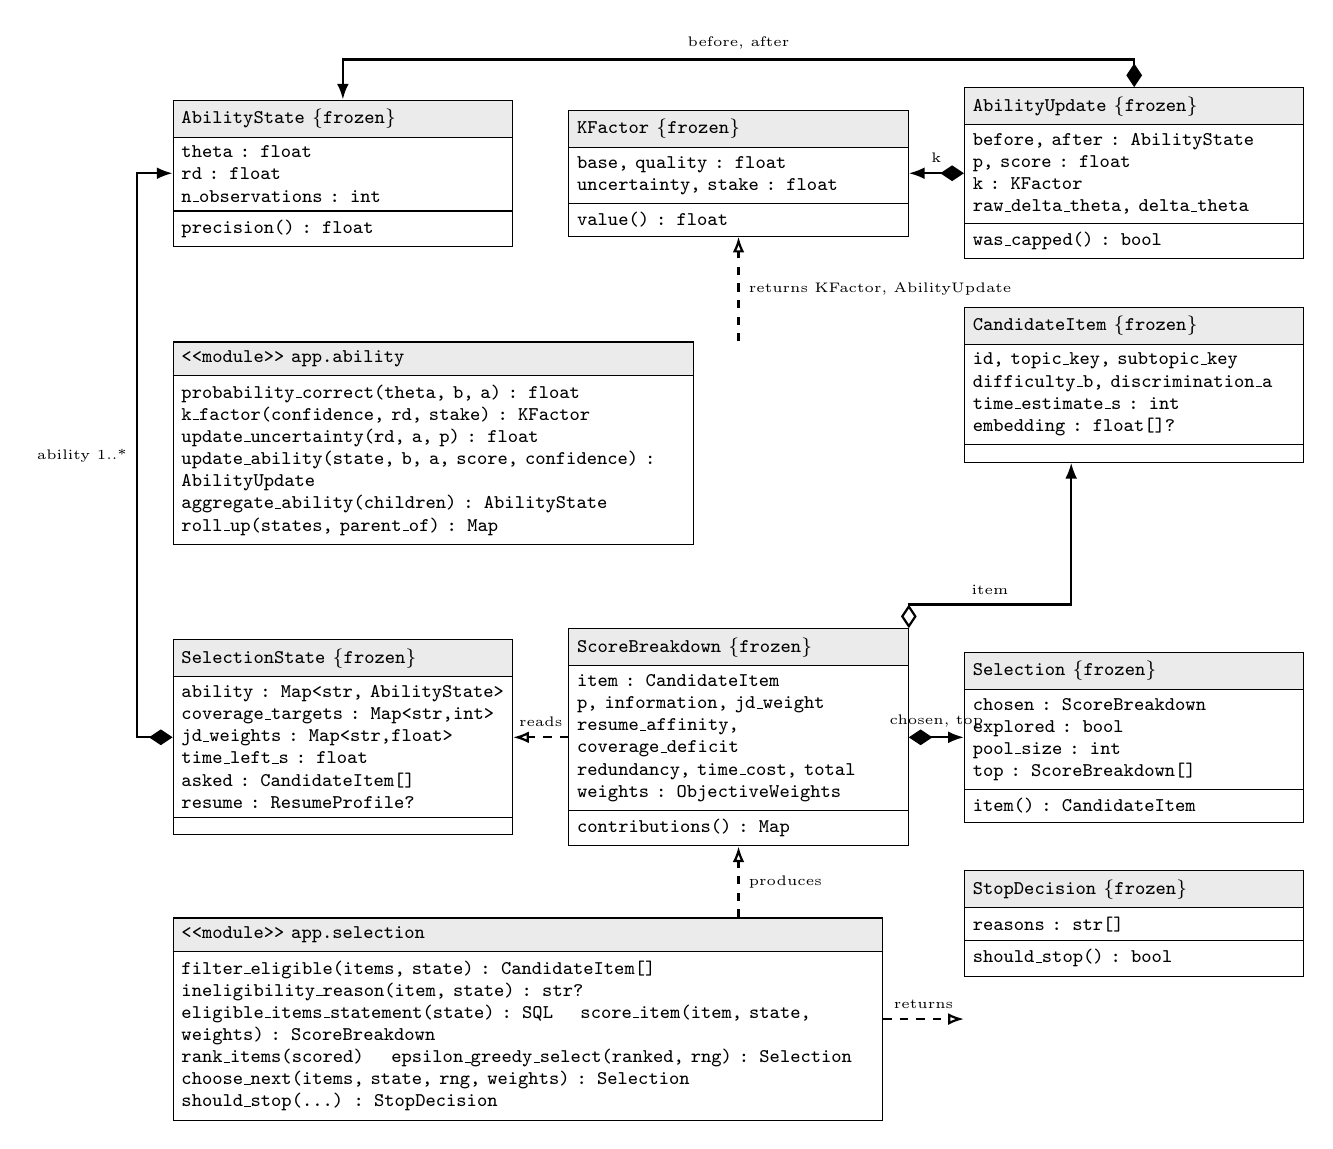
\begin{tikzpicture}[node distance=6mm and 7mm]
  \node[umlclass] (state) {\textbf{AbilityState} \{frozen\}\nodepart{second} theta : float\\ rd : float\\ n\_observations : int\nodepart{third} precision() : float};
  \node[umlclass, right=of state] (kf) {\textbf{KFactor} \{frozen\}\nodepart{second} base, quality : float\\ uncertainty, stake : float\nodepart{third} value() : float};
  \node[umlclass, right=of kf] (upd) {\textbf{AbilityUpdate} \{frozen\}\nodepart{second} before, after : AbilityState\\ p, score : float\\ k : KFactor\\ raw\_delta\_theta, delta\_theta\nodepart{third} was\_capped() : bool};
  \node[umlclass=2, below=of state, text width=64mm, anchor=north west] (abmod) at ([yshift=-6mm]state.south west) {\textbf{<<module>> app.ability}\nodepart{second}
    probability\_correct(theta, b, a) : float\\ k\_factor(confidence, rd, stake) : KFactor\\ update\_uncertainty(rd, a, p) : float\\ update\_ability(state, b, a, score, confidence) : AbilityUpdate\\ aggregate\_ability(children) : AbilityState\\ roll\_up(states, parent\_of) : Map};
  \node[umlclass, below=of upd] (item) {\textbf{CandidateItem} \{frozen\}\nodepart{second} id, topic\_key, subtopic\_key\\ difficulty\_b, discrimination\_a\\ time\_estimate\_s : int\\ embedding : float[]?\nodepart{third}};
  \node[umlclass, below=of abmod, anchor=north west] (sstate) at ([yshift=-6mm]abmod.south west) {\textbf{SelectionState} \{frozen\}\nodepart{second} ability : Map<str, AbilityState>\\ coverage\_targets : Map<str,int>\\ jd\_weights : Map<str,float>\\ time\_left\_s : float\\ asked : CandidateItem[]\\ resume : ResumeProfile?\nodepart{third}};
  \node[umlclass, right=of sstate] (score) {\textbf{ScoreBreakdown} \{frozen\}\nodepart{second} item : CandidateItem\\ p, information, jd\_weight\\ resume\_affinity, coverage\_deficit\\ redundancy, time\_cost, total\\ weights : ObjectiveWeights\nodepart{third} contributions() : Map};
  \node[umlclass, right=of score] (sel) {\textbf{Selection} \{frozen\}\nodepart{second} chosen : ScoreBreakdown\\ explored : bool\\ pool\_size : int\\ top : ScoreBreakdown[]\nodepart{third} item() : CandidateItem};
  \node[umlclass, below=of sel] (stop) {\textbf{StopDecision} \{frozen\}\nodepart{second} reasons : str[]\nodepart{third} should\_stop() : bool};
  \node[umlclass=2, below=of sstate, text width=88mm, anchor=north west] (selmod) at (sstate.south west |- stop.north) {\textbf{<<module>> app.selection}\nodepart{second}
    filter\_eligible(items, state) : CandidateItem[] \quad ineligibility\_reason(item, state) : str?\\ eligible\_items\_statement(state) : SQL \quad score\_item(item, state, weights) : ScoreBreakdown\\ rank\_items(scored) \quad epsilon\_greedy\_select(ranked, rng) : Selection\\ choose\_next(items, state, rng, weights) : Selection \quad should\_stop(\ldots) : StopDecision};
  \draw[compose] (upd.west) -- node[above, font=\tiny] {k} (kf.east);
  \draw[compose] (upd.north) -- ++(0,0.35) -| node[pos=0.25, above, font=\tiny] {before, after} (state.north);
  \draw[depend] (abmod.north -| kf.south) -- node[right, font=\tiny] {returns KFactor, AbilityUpdate} (kf.south);
  \draw[compose] (sstate.west) -- ++(-0.45,0) |- node[pos=0.25, left, font=\tiny] {ability 1..*} (state.west);
  \draw[aggreg] (score.north east) -- ++(0,0.3) -| node[pos=0.25, above, font=\tiny] {item} ([xshift=-8mm]item.south);
  \draw[compose] (score.east) -- node[above, font=\tiny] {chosen, top} (sel.west);
  \draw[depend] (score.west) -- node[above, font=\tiny] {reads} (sstate.east);
  \draw[depend] (selmod.east) -- node[above, font=\tiny] {returns} (stop.west |- selmod.east);
  \draw[depend] (selmod.north -| score.south) -- node[right, font=\tiny] {produces} (score.south);
\end{tikzpicture}
\caption{Class diagram of the adaptive engine: the ability model (top) and item selection (bottom). \texttt{ObjectiveWeights} holds the six named constants of Eq.~\eqref{eq:objective}.}
\label{fig:class-engine}
\end{figure}

\begin{figure}[htbp]
\centering
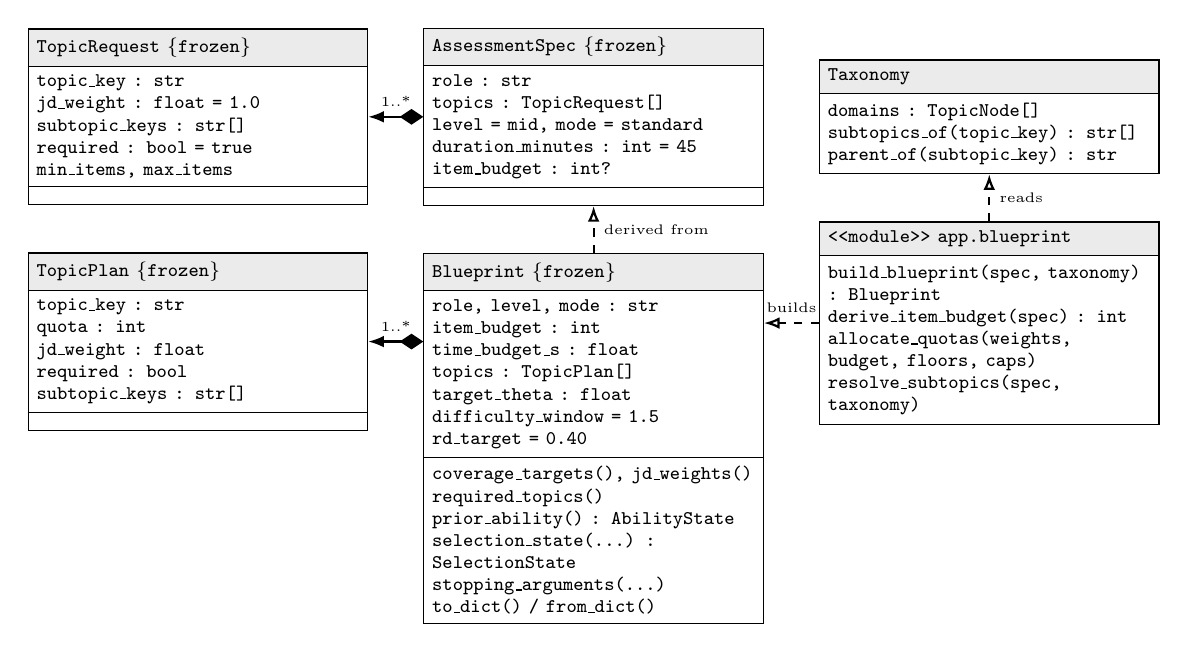
\begin{tikzpicture}[node distance=6mm and 7mm]
  \node[umlclass] (treq) {\textbf{TopicRequest} \{frozen\}\nodepart{second} topic\_key : str\\ jd\_weight : float = 1.0\\ subtopic\_keys : str[]\\ required : bool = true\\ min\_items, max\_items\nodepart{third}};
  \node[umlclass, right=of treq] (spec) {\textbf{AssessmentSpec} \{frozen\}\nodepart{second} role : str\\ topics : TopicRequest[]\\ level = mid, mode = standard\\ duration\_minutes : int = 45\\ item\_budget : int?\nodepart{third}};
  \node[umlclass=2, right=of spec] (tax) {\textbf{Taxonomy}\nodepart{second} domains : TopicNode[]\\ subtopics\_of(topic\_key) : str[]\\ parent\_of(subtopic\_key) : str};
  \node[umlclass, below=of treq] (tplan) {\textbf{TopicPlan} \{frozen\}\nodepart{second} topic\_key : str\\ quota : int\\ jd\_weight : float\\ required : bool\\ subtopic\_keys : str[]\nodepart{third}};
  \node[umlclass, below=of spec] (bp) {\textbf{Blueprint} \{frozen\}\nodepart{second} role, level, mode : str\\ item\_budget : int\\ time\_budget\_s : float\\ topics : TopicPlan[]\\ target\_theta : float\\ difficulty\_window = 1.5\\ rd\_target = 0.40\nodepart{third} coverage\_targets(), jd\_weights()\\ required\_topics()\\ prior\_ability() : AbilityState\\ selection\_state(...) : SelectionState\\ stopping\_arguments(...)\\ to\_dict() / from\_dict()};
  \node[umlclass=2, below=of tax] (bpmod) {\textbf{<<module>> app.blueprint}\nodepart{second} build\_blueprint(spec, taxonomy) : Blueprint\\ derive\_item\_budget(spec) : int\\ allocate\_quotas(weights, budget, floors, caps)\\ resolve\_subtopics(spec, taxonomy)};
  \draw[compose] (spec.west) -- node[above, font=\tiny] {1..*} (treq.east);
  \draw[compose] (bp.west |- tplan.east) -- node[above, font=\tiny] {1..*} (tplan.east);
  \draw[depend] (bpmod.north) -- node[right, font=\tiny] {reads} (tax.south);
  \draw[depend] (bpmod.west) -- node[above, font=\tiny] {builds} (bp.east |- bpmod.west);
  \draw[depend] (bp.north) -- node[right, font=\tiny] {derived from} (spec.south);
\end{tikzpicture}
\caption{Class diagram of the assessment blueprint. \texttt{AssessmentSpec} is the under-specified request; \texttt{Blueprint} the fully determined contract whose adapters produce the selector's inputs. \texttt{app.selection} never imports \texttt{app.blueprint}.}
\label{fig:class-blueprint}
\end{figure}

\begin{figure}[htbp]
\centering
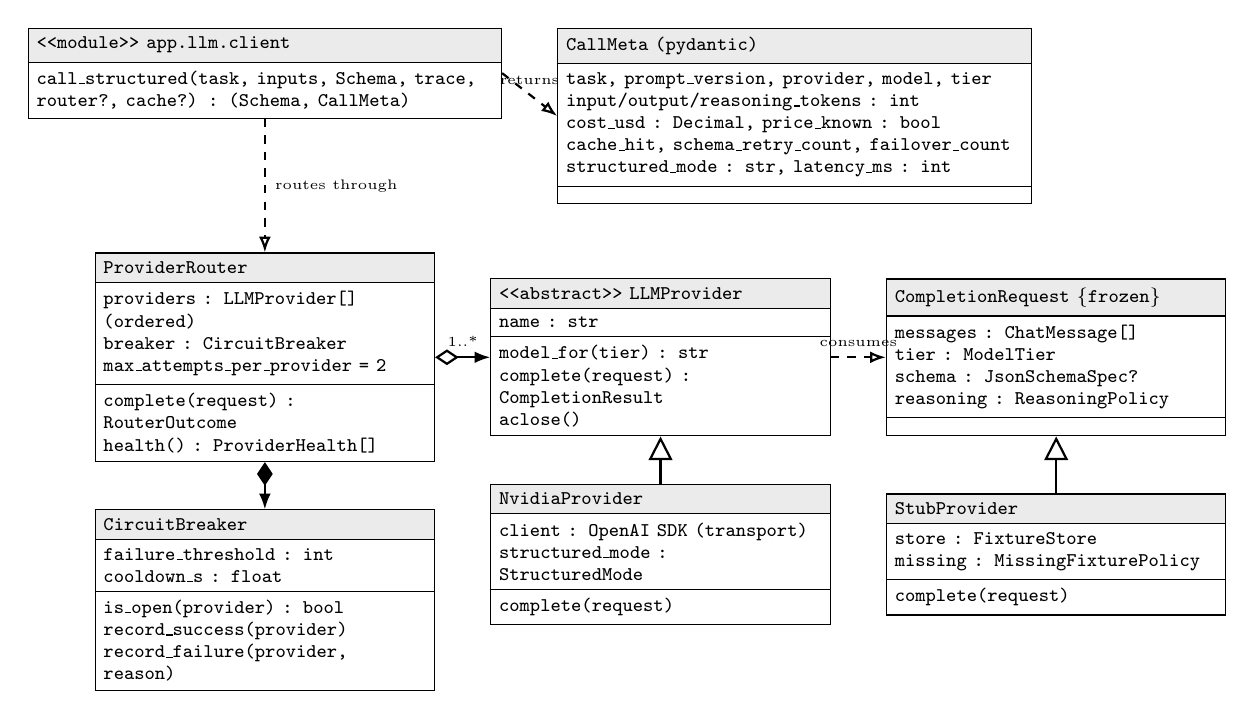
\begin{tikzpicture}[node distance=6mm and 7mm]
  \node[umlclass=2, text width=58mm] (cs) {\textbf{<<module>> app.llm.client}\nodepart{second} call\_structured(task, inputs, Schema, trace, router?, cache?) : (Schema, CallMeta)};
  \node[umlclass, anchor=north west, text width=58mm] at ([xshift=7mm]cs.north east) (meta) {\textbf{CallMeta} (pydantic)\nodepart{second} task, prompt\_version, provider, model, tier\\ input/output/reasoning\_tokens : int\\ cost\_usd : Decimal, price\_known : bool\\ cache\_hit, schema\_retry\_count, failover\_count\\ structured\_mode : str, latency\_ms : int\nodepart{third}};
  \node[umlclass, below=17mm of cs] (router) {\textbf{ProviderRouter}\nodepart{second} providers : LLMProvider[] (ordered)\\ breaker : CircuitBreaker\\ max\_attempts\_per\_provider = 2\nodepart{third} complete(request) : RouterOutcome\\ health() : ProviderHealth[]};
  \node[umlclass, right=of router] (prov) {\textbf{<<abstract>> LLMProvider}\nodepart{second} name : str\nodepart{third} model\_for(tier) : str\\ complete(request) : CompletionResult\\ aclose()};
  \node[umlclass, right=of prov] (req) {\textbf{CompletionRequest} \{frozen\}\nodepart{second} messages : ChatMessage[]\\ tier : ModelTier\\ schema : JsonSchemaSpec?\\ reasoning : ReasoningPolicy\nodepart{third}};
  \node[umlclass, below=of router] (breaker) {\textbf{CircuitBreaker}\nodepart{second} failure\_threshold : int\\ cooldown\_s : float\nodepart{third} is\_open(provider) : bool\\ record\_success(provider)\\ record\_failure(provider, reason)};
  \node[umlclass, below=of prov] (nv) {\textbf{NvidiaProvider}\nodepart{second} client : OpenAI SDK (transport)\\ structured\_mode : StructuredMode\nodepart{third} complete(request)};
  \node[umlclass, right=of nv] (stub) {\textbf{StubProvider}\nodepart{second} store : FixtureStore\\ missing : MissingFixturePolicy\nodepart{third} complete(request)};
  \draw[depend] (cs.south) -- node[right, font=\tiny] {routes through} (router.north);
  \draw[depend] (cs.east) -- node[above, font=\tiny] {returns} (meta.west);
  \draw[compose] (router.south) -- (breaker.north);
  \draw[aggreg] (router.east) -- node[above, font=\tiny] {1..*} (prov.west);
  \draw[depend] (prov.east) -- node[above, font=\tiny] {consumes} (req.west);
  \draw[inherit] (nv.north) -- (nv.north |- prov.south);
  \draw[inherit] (stub.north) -- (stub.north |- prov.south);
\end{tikzpicture}
\caption{Class diagram of the LLM chokepoint. \texttt{call\_structured} is the only entry point; \texttt{CallMeta} is the single record from which both the trace span and the cost report are projected; the NVIDIA adapter is the only class that knows the vendor exists.}
\label{fig:class-llm}
\end{figure}

\section{Activity Diagram}

Figure~\ref{fig:activity} is one adaptive interview session from a submitted specification to a
report -- UC-03 with UC-02 and UC-04 inlined, and exactly the loop the end-to-end test and the
simulation runner execute. Every decision node and every numeric update is in the engine lane;
the LLM lane holds only ``understand'', ``judge'' and ``speak'', each returning validated data
through the chokepoint. The \emph{any stop condition?} decision evaluates precision, item budget,
time budget and no-new-information and records every reason that holds; \emph{pool empty?} is
the one exit the stopping rule does not own -- the session ends with \texttt{pool\_exhausted}
rather than relaxing a constraint, because a constraint that can be relaxed is a penalty, and
penalties can be outweighed.

\begin{figure}[p]
\centering
\resizebox{!}{0.9\textheight}{%
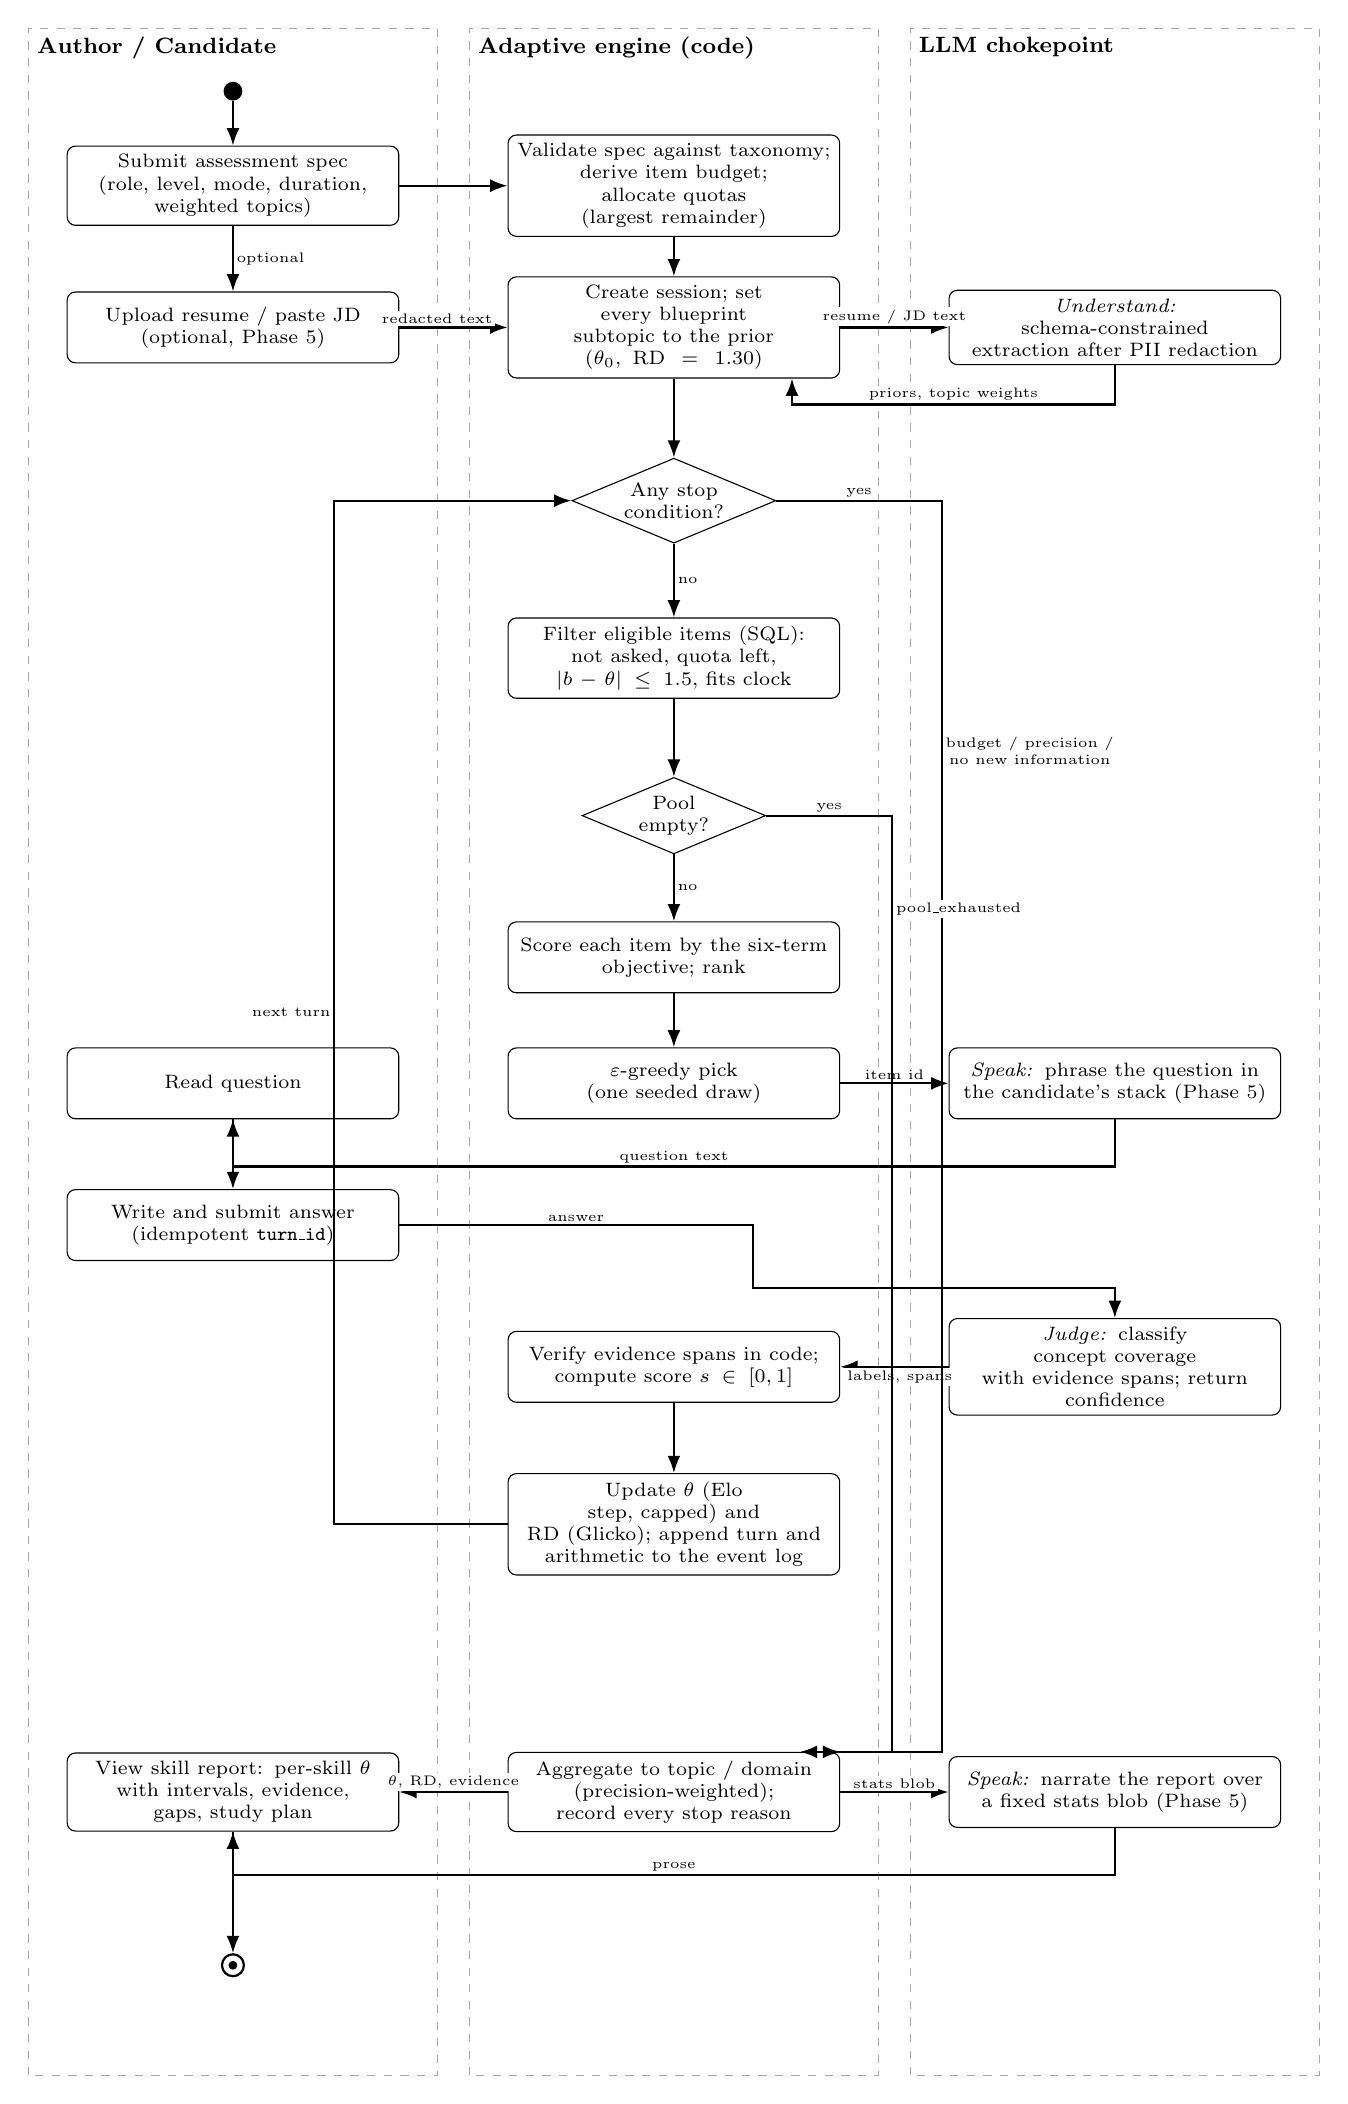
\begin{tikzpicture}[font=\scriptsize,
  act/.style={draw, rounded corners=3pt, align=center, inner sep=3pt, text width=40mm, minimum height=9mm, fill=white},
  dec/.style={draw, diamond, aspect=2.4, align=center, inner sep=1pt, fill=white},
  fl/.style={-{Latex[length=2.2mm]}, thick}, tag/.style={font=\tiny, fill=white, inner sep=1pt, align=center}]
  \def\A{0} \def\B{5.6} \def\C{11.2} \def\T{1.4} \def\Bot{-24.6}
  \begin{scope}[on background layer]
    \draw[swim] (\A-2.6,\Bot) rectangle (\A+2.6,\T);
    \draw[swim] (\B-2.6,\Bot) rectangle (\B+2.6,\T);
    \draw[swim] (\C-2.6,\Bot) rectangle (\C+2.6,\T);
  \end{scope}
  \node[swimlabel] at (\A-2.6,\T) {Author / Candidate};
  \node[swimlabel] at (\B-2.6,\T) {Adaptive engine (code)};
  \node[swimlabel] at (\C-2.6,\T) {LLM chokepoint};
  \node[circle, fill=black, inner sep=2.4pt] (start) at (\A,0.6) {};
  \node[act] (spec)   at (\A,-0.6)  {Submit assessment spec\\(role, level, mode, duration,\\weighted topics)};
  \node[act] (upload) at (\A,-2.4)  {Upload resume / paste JD\\(optional, Phase~5)};
  \node[act] (parse)  at (\C,-2.4)  {\emph{Understand:} schema-constrained\\extraction after PII redaction};
  \node[act] (build)  at (\B,-0.6)  {Validate spec against taxonomy;\\derive item budget;\\allocate quotas (largest remainder)};
  \node[act] (init)   at (\B,-2.4)  {Create session; set every blueprint\\subtopic to the prior $(\theta_0,\ \mathrm{RD}=1.30)$};
  \node[dec] (stopq)  at (\B,-4.6)  {Any stop\\condition?};
  \node[act] (elig)   at (\B,-6.6)  {Filter eligible items (SQL):\\not asked, quota left,\\$|b-\theta|\le 1.5$, fits clock};
  \node[dec] (poolq)  at (\B,-8.6)  {Pool\\empty?};
  \node[act] (scoreit) at (\B,-10.4) {Score each item by the six-term\\objective; rank};
  \node[act] (pick)   at (\B,-12.0) {$\varepsilon$-greedy pick\\(one seeded draw)};
  \node[act] (render) at (\C,-12.0) {\emph{Speak:} phrase the question in\\the candidate's stack (Phase~5)};
  \node[act] (show)   at (\A,-12.0) {Read question};
  \node[act] (answer) at (\A,-13.8) {Write and submit answer\\(idempotent \texttt{turn\_id})};
  \node[act] (grade)  at (\C,-15.6) {\emph{Judge:} classify concept coverage\\with evidence spans; return\\confidence};
  \node[act] (verify) at (\B,-15.6) {Verify evidence spans in code;\\compute score $s\in[0,1]$};
  \node[act] (update) at (\B,-17.6) {Update $\theta$ (Elo step, capped) and\\RD (Glicko); append turn and\\arithmetic to the event log};
  \node[act] (aggr)   at (\B,-21.0) {Aggregate to topic / domain\\(precision-weighted);\\record every stop reason};
  \node[act] (report) at (\C,-21.0) {\emph{Speak:} narrate the report over\\a fixed stats blob (Phase~5)};
  \node[act] (view)   at (\A,-21.0) {View skill report: per-skill $\theta$\\with intervals, evidence,\\gaps, study plan};
  \node[circle, draw, thick, inner sep=2.8pt] (end) at (\A,-23.2) {};
  \fill (end.center) circle (1.6pt);
  \draw[fl] (start) -- (spec);
  \draw[fl] (spec) -- (build);
  \draw[fl] (build) -- (init);
  \draw[fl] (spec) -- node[tag, right] {optional} (upload);
  \draw[fl] (upload.east) -- node[tag, above, pos=0.35] {redacted text} (init.west);
  \draw[fl] (init.east) -- node[tag, above] {resume / JD text} (parse.west);
  \draw[fl] (parse.south) -- ++(0,-0.5) -| node[tag, above, pos=0.25] {priors, topic weights} ([xshift=1.5cm]init.south);
  \draw[fl] (init) -- (stopq);
  \draw[fl] (stopq) -- node[tag, right] {no} (elig);
  \draw[fl] (elig) -- (poolq);
  \draw[fl] (poolq) -- node[tag, right] {no} (scoreit);
  \draw[fl] (scoreit) -- (pick);
  \draw[fl] (pick.east) -- node[tag, above] {item id} (render.west);
  \draw[fl] (render.south) -- ++(0,-0.6) -| node[tag, above, pos=0.25] {question text} (show.south);
  \draw[fl] (show) -- (answer);
  \draw[fl] (answer.east) -| node[tag, above, pos=0.25] {answer} (\B+1.0,-14.6) -| (grade.north);
  \draw[fl] (grade.west) -- node[tag, below, pos=0.45] {labels, spans} (verify.east);
  \draw[fl] (verify) -- (update);
  \draw[fl] (update.west) -- ++(-2.2,0) |- node[tag, left, pos=0.25] {next turn} (stopq.west);
  \draw[fl] (stopq.east) -- node[tag, above] {yes} ++(2.1,0) |- node[tag, right, pos=0.1] {budget / precision /\\no new information} ([xshift=2.1cm]aggr.north) -- (aggr.north east);
  \draw[fl] (poolq.east) -- node[tag, above] {yes} ++(1.6,0) |- node[tag, right, pos=0.05] {pool\_exhausted} ([xshift=1.6cm]aggr.north);
  \draw[fl] (aggr.east) -- node[tag, above] {stats blob} (report.west);
  \draw[fl] (report.south) -- ++(0,-0.6) -| node[tag, above, pos=0.25] {prose} (view.south);
  \draw[fl] (aggr.west) -- node[tag, above] {$\theta$, RD, evidence} (view.east);
  \draw[fl] (view.south) -- ++(0,-0.6) -| (end.north);
\end{tikzpicture}}
\caption{Activity diagram of one adaptive interview session. Decisions and every numeric update are in the engine lane; the LLM lane contains only understand, judge and speak. Actions marked Phase~5 are the parts the session layer will add; the engine-lane loop is implemented and is what the simulation runs.}
\label{fig:activity}
\end{figure}

{\renewcommand*{\bibfont}{\footnotesize}\printbibliography[heading=bibintoc]}
\end{document}
